%%%%%%%%%%%%%%%%%%%%%%%%%%%%%%%%%%%%%%%%%%%%%%%%%%%
%
%  New template code for TAMU Theses and Dissertations starting Fall 2012.  
%  For more info about this template or the 
%  TAMU LaTeX User's Group, see http://www.howdy.me/.
%
%  Author: Wendy Lynn Turner 
%	 Version 1.0 
%  Last updated 8/5/2012
%
%%%%%%%%%%%%%%%%%%%%%%%%%%%%%%%%%%%%%%%%%%%%%%%%%%%
%%%   Chapter - Transport
%%%%%%%%%%%%%%%%%%%%%%%%%%%%%%%%%%%%%%%%%%%%%%%%%%%
\chapter{\uppercase {The DGFEM Formulation of the Multigroup $S_N$ Equations}}
\label{sec::Sn}

%%%%%%%%%%%%%%%%%%%%%%%%%%%%%%%%%%%%%%%%%%%%%%%%%%%
%%%%%%%%%%%%%%%%%%%%%%%%%%%%%%%%%%%%%%%%%%%%%%%%%%%
%%%   Section - Introduction
%%%%%%%%%%%%%%%%%%%%%%%%%%%%%%%%%%%%%%%%%%%%%%%%%%%
%%%%%%%%%%%%%%%%%%%%%%%%%%%%%%%%%%%%%%%%%%%%%%%%%%%
\section{Fundamental Aspects of the Transport Equation}
\label{sec::DSA_aspects}

The movement of bulk materials and particles through some medium can be described by the statistical behavior of a non-equilibrium system. Boltzmann first devised these probabilistic field equations to characterize fluid flow via driving temperature gradients \cite{encyc_physics}. His work was later extended to model general fluid flow, heat conduction, Hamiltonian mechanics, quantum theory, general relativity, and radiation transport, among others. The Boltzmann Equation can be written in the general form:

\begin{equation}
\label{eq::gen_boltzmann}
\frac{\partial u}{\partial t} = \left( \frac{\partial u}{\partial t}  \right)_{force} + \left( \frac{\partial u}{\partial t}  \right)_{advec} + \left( \frac{\partial u}{\partial t}  \right)_{coll}
\end{equation}

\noindent where $u(\vec{r},\vec{p},t)$ is the transport distribution function parameterized in terms of position, $\vec{r}=(x,y,z)$, momentum, $\vec{p}=(p_x,p_y,p_z)$, and time, $t$. In simplified terms, Eq. (\ref{eq::gen_boltzmann}) can be interpreted that the time rate of the change of the distribution function, $\frac{\partial u}{\partial t}$, is equal to the sum of the change rates due to external forces, $\left( \frac{\partial u}{\partial t}  \right)_{force} $, advection of the particles, $\left( \frac{\partial u}{\partial t}  \right)_{advec}$, and particle-to-particle and particle-to-matter collisions, $\left( \frac{\partial u}{\partial t}  \right)_{coll}$ \cite{mcgraw_physics}. 

For neutral particle transport, the following assumptions \cite{duderstadt1979transport} about the behavior of the radiation particles can be utilized:

\begin{enumerate}
	\item Particles may be considered as points;
	\item Particles do not interact with other particles;
	\item Particles interact with material target atoms in a binary manner;
	\item Collisions between particles and material target atoms are instantaneous;
	\item Particles do not experience any external force fields ({\em e.g.,} gravity).
\end{enumerate}

These assumptions lead to the first-order form of the Boltzmann Transport Equation, which we simply call the transport equation for brevity. The remainder of the chapter is outlined as follows. Section \ref{sec::Sn_neut} provides the general form of the neutron transport equation with some variants. Section \ref{sec::Sn_MG} describes how we discretize the transport equation in energy with the multigroup methodology, and Section \ref{sec::Sn_Angle} presents the angular discretization via collocation. Section \ref{sec::Sn_BC} details which boundary conditions will be employed for our work. Section \ref{sec::Sn_Spatial} will conclude our discretization procedures in the spatial domain. Section \ref{sec::Sn_Solution} will present the iterative procedures used to obtain a numerical solution. We then present concluding remarks for the chapter in Section \ref{sec::Sn_Conclusions}.

%%%%%%%%%%%%%%%%%%%%%%%%%%%%%%%%%%%%%%%%%%%%%%%%%%%
%%%   Section - Neutron Transport Equation
\section{The Neutron Transport Equation}
\label{sec::Sn_neut}

The time-dependent neutron angular flux, $\Psi (\vec{r}, E, \vec{\Omega}, t)$, at spatial position $\vec{r}$, with energy $E$ moving in direction $\vec{\Omega}$ and at time $t$, is defined within an open, convex spatial domain $\mathcal{D}$, with boundary, $\partial \mathcal{D}$, by the general neutron transport equation:


\begin{equation}
\label{eq::Sn_transport_eq_full}
\begin{aligned}
\frac{1}{v(E)}\frac{\partial \Psi}{\partial t} + \vec{\Omega} \cdot \vec{\nabla} \Psi (\vec{r}, E, \vec{\Omega},t)+ \sigma_t (\vec{r}, E,t) \Psi (\vec{r}, E, \vec{\Omega},t) =Q_{ext} (\vec{r}, E, \vec{\Omega},t) \\
+ \frac{\chi (\vec{r}, E,t)}{4 \pi} \int dE' \nu \sigma_f (\vec{r}, E',t) \int d\Omega' \Psi (\vec{r}, E', \vec{\Omega}',t) \\ 
+ \int dE' \int d\Omega' \sigma_s (\vec{r},E' \rightarrow E, \Omega' \rightarrow \Omega,t) \Psi (\vec{r}, E', \vec{\Omega}',t)
\end{aligned}
\end{equation}

\noindent with the following, general boundary condition:

\begin{equation}
\label{eq::Sn_transport_bc_full}
\begin{aligned}
	\Psi (\vec{r}, E, \vec{\Omega},t) = \Psi^{inc} (\vec{r}, E, \vec{\Omega},t) + \int dE' \int d\Omega' \gamma (\vec{r}, E' \rightarrow E, \vec{\Omega}' \rightarrow \vec{\Omega},t) \Psi (\vec{r}, E', \vec{\Omega}',t) \\
	\text{for } \vec{r} \in \partial \mathcal{D}^{-} \left\{   \partial \mathcal{D}, \vec{\Omega} \cdot \vec{n} < 0  \right\}
\end{aligned} .
\end{equation}

\noindent In Eqs. (\ref{eq::Sn_transport_eq_full}) and (\ref{eq::Sn_transport_bc_full}), the physical properties of the system are defined as the following: $\sigma_t (\vec{r}, E,t)$ is the total neutron cross section, $\chi (\vec{r}, E,t)$ is the neutron fission spectrum, $\sigma_f (\vec{r}, E',t)$ is the fission cross section, $\nu (\vec{r}, E',t)$ is the average number of neutrons emitted per fission, $\sigma_s (E' \rightarrow E, \Omega' \rightarrow \Omega,t)$ is the differential scattering cross section, $Q_{ext} (\vec{r}, E, \vec{\Omega},t)$ is a distributed external source, $\Psi^{inc} (\vec{r}, E, \vec{\Omega},t)$ is the incident boundary source, and $\gamma (\vec{r}, E' \rightarrow E, \vec{\Omega}' \rightarrow \vec{\Omega},t)$ is the boundary albedo. We note that we have omitted the delayed neutron precursors from Eq. (\ref{eq::Sn_transport_eq_full}) because our work is restricted to steady-state problems.

We define the operator notation of Eq. (\ref{eq::Sn_transport_eq_full}):

\begin{equation}
\label{eq::Sn_transport_eq_op}
	\frac{1}{{\bf v}} \frac{\partial \Psi}{\partial t} + {\bf L} \Psi =  {\bf F} \Psi  + {\bf S} \Psi + {\bf Q},
\end{equation}

\noindent by dropping the dependent variable parameters and using the following operators:

\begin{equation}
\label{eq::Sn_transport_operators}
\begin{aligned}
	{\bf L} \Psi &= \vec{\Omega} \cdot \vec{\nabla} \Psi (\vec{r}, E, \vec{\Omega},t)+ \sigma_t (\vec{r}, E,t) \Psi (\vec{r}, E, \vec{\Omega},t), \\
	{\bf F} \Psi &= \frac{\chi (\vec{r}, E,t)}{4 \pi} \int dE' \nu \sigma_f (\vec{r}, E',t) \int d\Omega' \Psi (\vec{r}, E', \vec{\Omega}',t), \\
	{\bf S} \Psi &= \int dE' \int d\Omega' \sigma_s (E' \rightarrow E, \Omega' \rightarrow \Omega, t) \Psi (\vec{r}, E', \vec{\Omega}', t),  \\
	{\bf Q}       & = Q_{ext} (\vec{r}, E, \vec{\Omega},t) ,
\end{aligned}
\end{equation}

\noindent where ${\bf L}$ is the loss operator which includes total reaction and streaming, ${\bf F}$ is the fission operator, and ${\bf S}$ is the scattering operator. If we wish to analyze a transport problem at steady-state conditions, we simply omit the temporal derivative to form

\begin{equation}
\label{eq::Sn_transport_eq_op_SS}
	 {\bf L} \Psi =  {\bf F} \Psi  + {\bf S} \Psi + {\bf Q},
\end{equation}

\noindent and note that the operators of Eq. (\ref{eq::Sn_transport_operators}) no longer depend on time, $t$.

There is a special subset of transport problems that is routinely analyzed to determine the neutron behavior of a fissile system called the {\em k-eigenvalue problem}. In Eq. (\ref{eq::Sn_transport_eq_full}), $\nu (\vec{r}, E)$ acts as a multiplicative factor on the number of neutrons emitted per fission event. We replace this multiplicative factor in the following manner:

\begin{equation}
\label{eq::Sn_nubar_k}
	\nu (\vec{r}, E) \rightarrow \frac{{\nu} (\vec{r}, E)}{k},
\end{equation}

\noindent where we have introduced the eigenvalue, $k$. By also dropping the external source term, the steady-state neutron transport equation in Eq. (\ref{eq::Sn_transport_eq_op_SS}) can be rewritten into

\begin{equation}
\label{eq::Sn_transport_eq_op_keff}
	\left( {\bf L}  - {\bf S} \right) \tilde{\Psi} =  \frac{1}{k} {\bf F} \tilde{\Psi} ,
\end{equation}

\noindent where $(k, \tilde{\Psi})$ forms an appropriate eigenvalue-eigenvector pair. Of most interest is the eigenpair corresponding to the eigenvalue of largest magnitude.

We can then gain knowledge of the behavior of the neutron population in the problem by taking the full phase-space integrals of the left-hand-side and right-hand-side operators of Eq. (\ref{eq::Sn_transport_eq_op_keff}). With the appropriate eigenvector solution, $\tilde{\Psi}$, the $k$ eigenvalue then has the meaning as the multiplicative value which balances Eq. (\ref{eq::Sn_transport_eq_op_keff}) in an integral sense. This means that $k$ also has a physical meaning as well. A value $k<1$ is called subcritical and corresponds to a system whose neutron population decreases in time; a value $k=1$ is called critical and corresponds to a system whose neutron population remains constant in time; and a value $k>1$ is called supercritical and corresponds to a system whose neutron population increases in time \cite{ott1989}.


%%%%%%%%%%%%%%%%%%%%%%%%%%%%%%%%%%%%%%%%%%%%%%%%%%%
%%%   Section - Energy Discretization
\section{Energy Discretization}
\label{sec::Sn_MG}

We begin our discretization procedures by focusing on the angular flux's energy variable. An ubiquitous energy discretization procedure in the transport community is the multigroup method \cite{duderstadt1976nuclear,lewis1984computational}. The multigroup method is defined by splitting the angular flux solution into $G$ number of distinct, contiguous, and non-overlapping energy intervals called groups. We begin by restricting the full energy domain, $[0, \infty)$, into a finite domain, $E \in [E_G, E_0]$. $E_0$ corresponds to some maximum energy value and $E_G$ corresponds to some minimum energy value (typically 0). We have done this by defining $G+1$ discrete energy values that are in a monotonically continuous reverse order: $E_G < E_{G-1} <  \ldots < E_1 < E_0$. 

From this distribution of energy values, we then say that a particular energy group, $g$, corresponds to the following energy interval:

\begin{equation}
\label{eq::Sn_MG_energy_interval}
\Delta E_g \in [E_g, E_{g-1}].
\end{equation}

\noindent Figure \ref{fig::Sn_MG_energy_bands} provides a visual representation between the $G+1$ discrete energy values and the $G$ energy groups. While the order that we have prescribed may seem illogical (high-to-low) to those outside of the radiation physics community, it has been historically applied this way because radiation transport problems are iteratively solved from high energy to low energy.

\begin{figure}[bht]
\centering
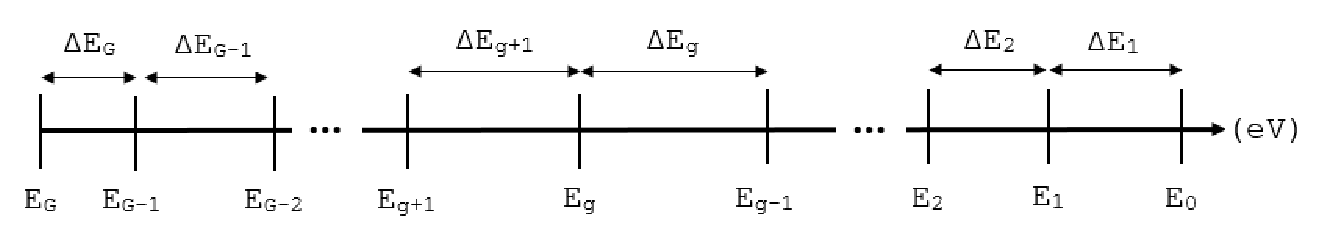
\includegraphics[width=0.975\textwidth]{figures/sec_Sn/MG_Energy_Bands.eps}
\caption{Interval structure of the multigroup methodology.}
\label{fig::Sn_MG_energy_bands}
\end{figure}

For the remainder of this energy discretization procedure, we will utilize the steady-state form of the transport equation in Eq. (\ref{eq::Sn_transport_eq_op_SS}). The time-dependent and eigenvalue forms are analogous and would be derived identically. Taking the energy interval for group $g$ as defined in Eq. (\ref{eq::Sn_MG_energy_interval}), the energy-integrated angular flux of group $g$ is

\begin{equation}
\label{eq::Sn_MG_ang_flux_g}
\Psi_g (\vec{r}, \vec{\Omega}) = \int_{E_g}^{E_{g-1}} \, \Psi (\vec{r}, E, \vec{\Omega}) \, dE .
\end{equation}

\noindent We can then use the energy-integrated angular flux to form the following coupled, $(g=1,...,G)$, discrete equations (we have dropped the spatial parameter and some of the angular parameters for further clarity):

\begin{equation}
\label{eq::Sn_MG_trans_eq}
\left(  \vec{\Omega} \cdot \vec{\nabla} + \sigma_{t,g}  \right) \Psi_g =  \sum_{g'=1}^{G} \left[ \frac{\chi_g}{4 \pi} \nu \sigma_{f,g'} \int_{4 \pi} \Psi_{g'} (\vec{\Omega}') \, d\Omega' + \int_{4 \pi} \sigma_{s}^{g' \rightarrow g} (\vec{\Omega}' , \vec{\Omega} ) \Psi_{g'} (\vec{\Omega}')  \, d\Omega'  \right] + Q_g
\end{equation}

\noindent where

\begin{equation}
\label{eq::Sn_MG_exact_condensed_terms}
\begin{aligned}
\sigma_{t,g} (\vec{r}) & \equiv \frac{\int_{E_{g}}^{E_{g-1}} \sigma_{t} (\vec{r},E) \int_{4 \pi} \Psi (\vec{r},\vec{\Omega}, E) \, dE d\Omega}{\int_{E_{g}}^{E_{g-1}} \int_{4 \pi} \Psi (\vec{r},\vec{\Omega}, E) \, dE d\Omega}\\
\nu\sigma_{f,g} (\vec{r}) & \equiv \frac{\int_{E_{g}}^{E_{g-1}} \nu\sigma_{f} (\vec{r},E)  \int_{4 \pi} \Psi (\vec{r},\vec{\Omega}, E) \, dE d\Omega}{\int_{E_{g}}^{E_{g-1}} \int_{4 \pi} \Psi (\vec{r},\vec{\Omega}, E) \, dE d\Omega} \\
\chi_g & \equiv \int_{E_{g}}^{E_{g-1}} \chi  (\vec{r},E) \, dE \\
\sigma_{s}^{g' \rightarrow g} (\vec{r},\vec{\Omega}' , \vec{\Omega} ) & \equiv \frac{\int_{E_{g'}}^{E_{g'-1}} \left[ \int_{E_{g}}^{E_{g-1}} \sigma_s (\vec{r},E' \rightarrow E,\vec{\Omega}' , \vec{\Omega} ) \, dE \right] \Psi (\vec{r},\vec{\Omega}', E') \, dE' }{\int_{E_{g'}}^{E_{g'-1}}  \Psi (\vec{r},\vec{\Omega}, E) \, dE} \\
Q_g (\vec{r}, \vec{\Omega}) & \equiv \int_{E_{g}}^{E_{g-1}} Q (\vec{r}, \vec{\Omega}, E) \, dE
\end{aligned}
\end{equation}

The above equations are mathematically exact to those presented in Eqs. (\ref{eq::Sn_transport_eq_full} - \ref{eq::Sn_transport_eq_op_SS}), and we have made no approximations at this time. However, this requires full knowledge of the energy distribution of the angular flux solution at all positions in our problem domain since we weight the multigroup cross sections with this solution. This is obviously impossible since the energy distribution is part of the solution space for which we are trying to solve. Instead, we now define the process to make the multigroup discretization an effective approximation method.

We first define an approximate angular flux distribution for a region $s$:

\begin{equation}
\label{eq::Sn_MG_flux_approx}
\Psi (\vec{r},\vec{\Omega}, E) =  \hat{\Psi} (\vec{r},\vec{\Omega}) f_{s} (E) ,
\end{equation}

\noindent which is a factorization of the angular flux solution into a region-dependent energy function, $f_s (E)$, and a spatially/angularly dependent function, $\hat{\Psi} (\vec{r},\vec{\Omega})$. With this approximation, we can redefine the energy-collapsed cross sections of Eq. (\ref{eq::Sn_MG_exact_condensed_terms}):

\begin{equation}
\label{eq::MG_approx_condensed_terms}
\begin{aligned}
\sigma_{t,g} (\vec{r}) & \equiv \frac{\int_{E_{g}}^{E_{g-1}} \sigma_{t} (\vec{r},E) f_{s} (E) \, dE}{\int_{E_{g}}^{E_{g-1}} f_{s} (E) \, dE} ,\\
\nu\sigma_{f,g} (\vec{r}) & \equiv \frac{\int_{E_{g}}^{E_{g-1}} \nu\sigma_{f} (\vec{r},E)  f_{s} (E) \, dE }{\int_{E_{g}}^{E_{g-1}} f_{s} (E) \, dE}, \\
\sigma_{s}^{g' \rightarrow g} (\vec{r},\vec{\Omega}' , \vec{\Omega} ) & \equiv \frac{\int_{E_{g'}}^{E_{g'-1}} \left[ \int_{E_{g}}^{E_{g-1}} \sigma_s (\vec{r},E' \rightarrow E,\vec{\Omega}' , \vec{\Omega} ) \, dE \right] f_{s} (E')\, dE' }{\int_{E_{g'}}^{E_{g'-1}}  f_{s} (E) \, dE} .
\end{aligned}
\end{equation}

\noindent It is noted that we do not need to redefine the fission spectrum or the distributed external sources since they are not weighted with the angular flux solution. With this energy factorization, we would expect, in general, that the approximation error will tend to zero as the number of discrete energy groups increases (thereby making the energy bins thinner). This is especially true if the group structure is chosen with many more bins in energy regions with large variations in the energy solution. For certain problems, the region-dependent energy function is well understood ({\em i.e.,} almost exactly known). This means that, for these problems, we can achieve reasonable solution accuracy with only a few groups where the energy bins of the multigroup discretization are well chosen.

%%%%%%%%%%%%%%%%%%%%%%%%%%%%%%%%%%%%%%%%%%%%%%%%%%%
%%%   Section - Angle Discretization
\section{Angular Discretization}
\label{sec::Sn_Angle}

Now that we have provided the discretization of the energy variable, we next focus on the discretization of the transport problem in angle. We will do this in two stages: 1) expand the scattering source and the distributed external source in spherical harmonics and 2) collocate the angular flux at the interpolation points of the angular trial space. We will perform these discretization procedures by taking the steady-state equation presented in Eq. (\ref{eq::Sn_transport_eq_op_SS}), dropping spatial parameterization, combining the fission and external sources into a single term, and using only 1 energy group:

\begin{equation}
\label{eq::Sn_Angle_simple_trans_eq}
\vec{\Omega} \cdot \vec{\nabla} \Psi (\vec{\Omega}) + \sigma_t \Psi (\vec{\Omega}) = \int_{4 \pi}  d\Omega' \, \sigma_s ( \vec{\Omega}' \rightarrow \vec{\Omega}) \Psi (\vec{\Omega}') + Q  (\vec{\Omega}) .
\end{equation}

We first develop an approximation for the scattering term in Eq. (\ref{eq::Sn_Angle_simple_trans_eq}) by expanding the angular flux and the scattering cross section in spherical harmonics functions and Legendre polynomials, respectively. We begin by first assuming that the material is isotropic in relation to the radiation's initial direction. From this assumption, the parameterization of the scattering cross section can be written in terms of only the scattering angle, $\mu_0$,

\begin{equation}
\label{eq::Sn_scatt_xs}
\sigma_s ( \vec{\Omega}' \rightarrow \vec{\Omega}) = \frac{1}{2 \pi} \sigma_s ( \vec{\Omega}' \cdot \vec{\Omega}) = \frac{1}{2 \pi} \sigma_s ( \mu_0) , 
\end{equation}

\noindent where $\mu_0 \equiv  \vec{\Omega}' \cdot \vec{\Omega}$. With this assumption, the scattering cross section can now be expanded in an infinite series in terms of the Legendre polynomials,

\begin{equation}
\label{eq::Sn_scatt_xs_legendre}
\sigma_s ( \vec{\Omega}' \rightarrow \vec{\Omega}) = \sum\displaylimits_{p=0}^{\infty} \frac{2p + 1}{4 \pi}  \sigma_{s,p} P_p ( \mu_0) , 
\end{equation}

\noindent where $\sigma_{s,p}$ is the $p$ angular moment of the scattering cross section. These angular moments of the scattering cross section have the form:

\begin{equation}
\label{eq::Sn_scatt_xs_moments}
	\sigma_{s,p} \equiv  \int_{-1}^{1} \, d \mu_0 \, \sigma_s ( \mu_0) P_p (\mu_0)  .
\end{equation}

With the scattering cross section redefined, we can now expand the angular flux in terms of an infinite series of the spherical harmonics functions, $Y$,

\begin{equation}
\label{eq::Sn_ang_flux_sph_harm_funcs}
\Psi (\vec{\Omega}) = \frac{1}{4 \pi} \sum\displaylimits_{k=0}^{\infty} \sum\displaylimits_{n=-k}^{k} \Phi_{k,n} Y_{k,n} (\vec{\Omega})
\end{equation}

\noindent where the angular moments of the angular flux, $\Phi_{k,n}$, have the form:

\begin{equation}
\label{eq::Sn_flux_moments}
	\Phi_{k,n} \equiv \int_{4 \pi} d\Omega \, \Psi(\vec{\Omega}) \, Y_{k,n} (\vec{\Omega}).
\end{equation}

\noindent We note that the $p$ and $k$ orders of the scattering cross section and angular flux expansions, respectively, are not corresponding. We then take the scattering cross section expansion of Eq. (\ref{eq::Sn_scatt_xs_legendre}) and the angular flux expansion of Eq. (\ref{eq::Sn_ang_flux_sph_harm_funcs}) and insert them into the original scattering term of the right-hand-side of Eq. (\ref{eq::Sn_Angle_simple_trans_eq}). After significant algebra and manipulations, which we will not include here for brevity, the scattering term can be greatly simplified (the full details of this are located in Appendix \ref{sec::appendix_SN}). Eq. (\ref{eq::Sn_Angle_simple_trans_eq}) can now be written again with this alternate and simplified scattering term that is composed of the cross section and angular flux moments:

\begin{equation}
\label{eq::Sn_Angle_simple_trans_eq_w_moments_inf}
\vec{\Omega} \cdot \vec{\nabla} \Psi (\vec{\Omega}) + \sigma_t \Psi (\vec{\Omega}) = \sum_{p=0}^{\infty} \frac{2p + 1}{4 \pi} \sigma_{s,p}   \sum_{n=-p}^{p}  \Phi_{p,n}  Y_{p,n} (  \vec{\Omega} )+ Q  (\vec{\Omega}) .
\end{equation}

From the initial assumption of material isotropy (which may or may not be an approximation), the scattering term of Eq. (\ref{eq::Sn_Angle_simple_trans_eq_w_moments_inf}) has introduced no approximation. Unfortunately, this form requires an infinite series expansion which we cannot use with only finite computational resources. Instead, we truncate the series at some maximum expansion order, $N_p$, which, in general, introduces an approximate form for the scattering. However, we note that if the problem's scattering anisotropy can be exactly captured with moments through order $N_p$, then we have introduced no approximation with this truncation. With this order of truncation, we again write the angularly continuous Eq. (\ref{eq::Sn_Angle_simple_trans_eq_w_moments_inf}) but also fold the source term into the spherical harmonics expansion,

\begin{equation}
\label{eq::Sn_Angle_simple_trans_eq_w_moments_trunc}
\vec{\Omega} \cdot \vec{\nabla} \Psi (\vec{\Omega}) + \sigma_t \Psi (\vec{\Omega}) = \sum_{p=0}^{N_p} \frac{2p + 1}{4 \pi}   \sum_{n=-p}^{p}   Y_{p,n} (  \vec{\Omega} ) \left[ \sigma_{s,p} \Phi_{p,n} + Q_{p,n}  \right] .
\end{equation}

At this point, one may wonder why we have altered the scattering operator so that it is terms of moments of the scattering cross sections and the angular flux. The reason is two-fold which will also be discussed in further detail later in this chapter. First, it greatly simplifies the representation of the scattering cross sections. With proper preprocessing, the scattering cross sections can be simplified into just their Legendre moments, instead of having to store angle-to-angle quantities ($\vec{\Omega}' \rightarrow \vec{\Omega}$). For every group-to-group combination in energy ($g' \rightarrow g$), there are only the $N_p$ moments of the scattering cross section. Secondly, the contribution of the angular flux into the scattering source with its moments can also greatly reduce the dimensional space that needs to be stored in computer memory. This will be discussed later in further detail in Section \ref{sec::Sn_Solution_Iterative}, but it simply means that we only have to store $N_{mom}$ angular flux moments for use in the scattering source. In 1 dimension, $N_{mom}$ is equal to ($N_p + 1$). In 2 dimensions, $N_{mom}$ is equal to $\frac{(N_p + 1) (N_p + 2)}{2}$. In 3 dimensions, $N_{mom}$ is equal to $(N_p + 1)^2$. For comparative purposes, we have plotted $N_{mom}$ for 1, 2, and 3 dimensions up to order 8 in Figure \ref{fig::Sn_Num_Sph_Harm_Moments}.

\begin{figure}
\centering
\includegraphics[width=0.65\textwidth]{figures/sec_Sn/Num_Sph_Harm_Moments.eps}
\caption{Number of spherical harmonics moments, $N_{mom}$, in 1D, 2D, and 3D as a function of the expansion order, $p$.}
\label{fig::Sn_Num_Sph_Harm_Moments}
\end{figure}

Up to this point, we have only presented the methodology to express our source terms with expansions of the spherical harmonics functions. Next, we describe the second portion of our angular discretization by deriving the standard $S_N$ equations using a collocation technique. We begin by choosing a set of $M$ distinct points and weights to form a quadrature set in angular space: $\{  \vec{\Omega}_m, w_m \}_{m=1}^M$. We will give further details about the required characteristics of this quadrature set as well as a couple of common options a little later. Using this quadrature set, we can further define a trial space for the angular flux,

\begin{equation}
\label{eq::Sn_ang_flux_basis}
\Psi (\vec{\Omega}) = \sum\displaylimits_{m=1}^{M} B_m (\vec{\Omega})  \Psi_m ,
\end{equation}

\noindent where the angular bases, $B_m$, satisfy the {\em Kronecker} property,

\begin{equation}
\label{eq::Sn_ang_basis_kroneker}
 B_j (\vec{\Omega}_m) = \delta_{j,m}, 
\end{equation}

\noindent as well as the {\em Lagrange} property,

\begin{equation}
\label{eq::Sn_ang_basis_lagrange}
\sum\displaylimits_{m=1}^{M} B_m (\vec{\Omega}) = 1  ,
\end{equation}

\noindent and the singular value of the angular flux along a given direction has the following notation:

\begin{equation}
\label{eq::Sn_ang_flux_identity}
\Psi_m = \Psi (\vec{\Omega}_m).
\end{equation}

Next, we substitute Eq. (\ref{eq::Sn_ang_flux_basis}) into Eq. (\ref{eq::Sn_Angle_simple_trans_eq_w_moments_trunc}), drop the external source for brevity, and collocate at the ($k=1,...,M$) interpolation (quadrature) points,

\begin{equation}
\label{eq::Sn_Angle_simple_trans_eq_w_ang_basis}
\begin{aligned}
\vec{\Omega} \cdot \vec{\nabla} \left( \sum\displaylimits_{m=1}^{M} B_m (\vec{\Omega}_k)  \Psi_m \right) + \sigma_t \left(  \sum\displaylimits_{m=1}^{M} B_m (\vec{\Omega}_k)  \Psi_m \right) \\
= \sum_{p=0}^{N_p} \frac{2p + 1}{4 \pi} \sigma_{s,p}   \sum_{n=-p}^{p}   Y_{p,n} (  \vec{\Omega} ) \left(  \sum\displaylimits_{m=1}^M \Psi_m \int_{4 \pi} d\Omega \, B_m (\vec{\Omega}_k)  \, Y_{p,n} (\vec{\Omega})  \right)  \\
k=1,...,M
\end{aligned} ,
\end{equation}

\noindent where we inserted Eq. (\ref{eq::Sn_ang_flux_basis}) into Eq. (\ref{eq::Sn_flux_moments}) to form a slightly modified form for the angular flux moments:

\begin{equation}
\label{eq::Sn_flux_mom_int_w_basis}
\Phi_{p,n} = \sum\displaylimits_{m=1}^M \Psi_m \int_{4 \pi} d\Omega \, B_m (\vec{\Omega})  \, Y_{p,n} (\vec{\Omega}).
\end{equation}

\noindent The {\em Kronecker} property of Eq. (\ref{eq::Sn_ang_basis_kroneker}), is then used at the collocation points so that Eq. (\ref{eq::Sn_Angle_simple_trans_eq_w_ang_basis}) can be simplified into the following form (where we have reintroduced the distributed source term in terms of its contribution for angle $m$):

\begin{equation}
\label{eq::Sn_trans_eq_angle_disc_FINAL}
\begin{aligned}
\vec{\Omega}_m \cdot \vec{\nabla} \Psi_{m}  + \sigma_{t}   \Psi_{m}=  \sum_{p=0}^{N_P} \frac{2p + 1}{4 \pi}  \sigma_{s,p}  \sum_{n=-p}^{p}  Y_{p,n} (  \vec{\Omega}_m )  \Phi_{p,n}  + Q_{m}  \\
m=1,...,M
\end{aligned} .
\end{equation}

Equation (\ref{eq::Sn_trans_eq_angle_disc_FINAL}) represents the transport equation that has been discretized into $M$ separate equations in angle (for 1 energy group and no spatial discretization). Up to this point, we have simply stated that there is some angular quadrature set composed of $M$ directions and weights that will satisfy some conditions of the solution, but we have not explicitly stated these conditions. For this work, we will require our angular quadrature set to maintain the following properties:

\begin{enumerate}
\item The weights can sum to 1 by some normalization procedure: $\sum\displaylimits_m w_m = 1$.
\item The odd angular moments sum to $\vec{0}$: $\sum\displaylimits_m w_m \left( \vec{\Omega}_m  \right)^n =  \vec{0}$ ($n=1,3,5,...$).
\item $\sum\displaylimits_m w_m  \vec{\Omega}_m \vec{\Omega}_m = \frac{1}{3} \mathbb{I}  $, where $\mathbb{I}$ is the identity tensor.
\item The points and weights are symmetric about the primary axes in angular space. 
\item The points and weights also need to have symmetry about the problem domain boundary (this is not an issue if the domain is a rectangle in 2D or an orthogonal parallelepiped in 3D). This point is important for reflecting boundary conditions and is described in greater detail in Section \ref{sec::Sn_BC}.
\end{enumerate}

\noindent Point 4 requires some additional explanation. In 1 dimension, this corresponds to symmetry about the point 0 on the interval $[-1, 1]$. In 2 dimensions, this corresponds to quadrant-to-quadrant symmetry about the x-y primary axes of the unit circle. In 3 dimensions, this corresponds to octant-to-octant symmetry about the x-y-z primary axes of the unit sphere. 

From these properties, especially property 4, our 2D and 3D quadrature sets can be constructed in a simple and consistent manner (1D quadrature sets have different construction, and our work does not include them). For both 2D and 3D problems, we can generate a subset of the quadrature points and weights on a single octant of the unit sphere, where each quadrature point in this subset has the form: $\vec{\Omega} = [\mu, \eta , \xi]$ . If we are solving a 2D problem, we would then project the quadrature points onto the $(0 < \theta < \frac{\pi}{2})$ portion of the unit circle so that they have the form: $\vec{\Omega} = [\mu, \eta ]$ (we can then view the primary octant as the primary quadrant). Once we have defined the quadrature points and weights for the primary quadrant or octant, we can then directly calculate the remainder of the quadrature set by mapping to the other quadrants or octants. Table \ref{tab::Sn_2D_octant_mapping} presents the mapping from the primary quadrant to the other 3 quadrants for 2D problems. Table \ref{tab::Sn_3D_octant_mapping} presents the mapping from the primary octant to the other 7 octants for 3D problems. In these tables, the `1' subscript corresponds to those angles generated in the primary quadrant or octant.

\begin{table}[hbt]
\centering
\caption{2D angle mapping from the first quadrant into the other 3 quadrants.}
\begin{tabular}{|c|cc|}
	\hline
	Quadrant & $\mu$ & $\eta$ \\
	\hline
	1 & $\mu_1=\mu_1$ & $\eta_1=\eta_1$ \\
	\hline
	2 & $\mu_2=-\mu_1$ & $\eta_2=\eta_1$ \\
	\hline
	3 & $\mu_3=-\mu_1$ & $\eta_3=-\eta_1$ \\
	\hline
	4 & $\mu_4=\mu_1$ & $\eta_4=-\eta_1$ \\
	\hline
\end{tabular}
\label{tab::Sn_2D_octant_mapping}
\end{table}

\begin{table}[hbt]
\centering
\caption{3D angle mapping from the first octant into the other 7 octants.}
\begin{tabular}{|c|ccc|}
	\hline
	Octant & $\mu$ & $\eta$ & $\xi $ \\
	\hline
	1 & $\mu_1=\mu_1$ & $\eta_1=\eta_1$ & $\xi_1=\xi_1$ \\
	\hline
	2 & $\mu_2=-\mu_1$ & $\eta_2=\eta_1$ & $\xi_2=\xi_1$ \\
	\hline
	3 & $\mu_3=-\mu_1$ & $\eta_3=-\eta_1$ & $\xi_3=\xi_1$ \\
	\hline
	4 & $\mu_4=\mu_1$ & $\eta_4=-\eta_1$ & $\xi_4=\xi_1$ \\
	\hline
	5 & $\mu_5=\mu_1$ & $\eta_5=\eta_1$ & $\xi_5=-\xi_1$ \\
	\hline
	6 & $\mu_6=-\mu_1$ & $\eta_6=\eta_1$ & $\xi_6=-\xi_1$ \\
	\hline
	7 & $\mu_7=-\mu_1$ & $\eta_7=-\eta_1$ & $\xi_7=-\xi_1$ \\
	\hline
	8 & $\mu_8=\mu_1$ & $\eta_8=-\eta_1$ & $\xi_8=-\xi_1$ \\
	\hline
\end{tabular}
\label{tab::Sn_3D_octant_mapping}
\end{table}

We conclude our discussion of angular discretizations by presenting two common angular quadrature sets that will be employed in this dissertation work. Section \ref{sec::Sn_Angle_LS} presents the Level Symmetric (LS) quadrature set and Section \ref{sec::Sn_Angle_PGLC} presents the Product Gauss-Legendre-Chebyshev (PGLC) quadrature set. Both of these quadrature sets can be formed from the procedure outlined before: form the primary octant and then map appropriately.

%%%%%%%%%%%%%%%%%%%%%%%%%%%%%%%%%%%%%%%%%%%%%%%%%%%
%%%   SubSection - Level-Symmetric
\subsection{Level Symmetric Quadrature Set}
\label{sec::Sn_Angle_LS}

The first quadrature set we present is the common Level Symmetric set that has had extensive use in the radiation transport community \cite{lewis1984computational,carlson1968computing}. Its defining characteristic is the restriction that it is rotationally symmetric (invariant) about all three axes of the primary octant. This leads to a two-fold additional set of restrictions: 1) once the location of the first ordinate is selected, then all other ordinates are known; and 2) the weights can become negative. This negativity of the weights can be problematic and lead to unphysical solutions if the angular flux is not sufficiently smooth.

\begin{figure}
\centering
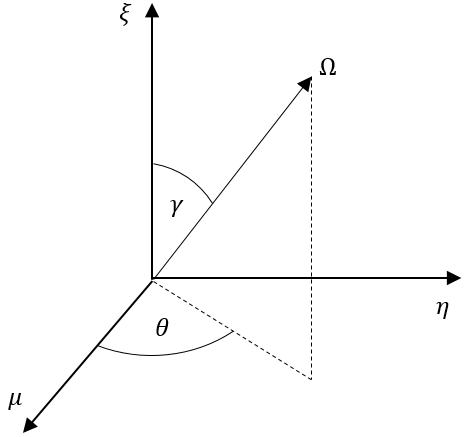
\includegraphics[width=0.45\textwidth]{figures/sec_Sn/Ang_Quad_Coord_Sys.png}
\caption{Angular coordinate system for the direction $\vec{\Omega}$.}
\label{fig::Ang_Coord_Sys}
\end{figure}

We begin our description of the LS quadrature by analyzing the 3D angular coordinate system for a particular direction, $\vec{\Omega}$, as depicted in Figure \ref{fig::Ang_Coord_Sys}. The angular direction, $\vec{\Omega} = [\vec{\Omega}_x, \vec{\Omega}_y, \vec{\Omega}_z]$, is typically described with its directional cosines: $\mu$, $\eta$, and $\xi$. These are described by the angles $\theta$ and $\gamma$ of the coordinate system, which are the azimuthal and polar angles, respectively, and allow us to give a functional form for each direction component:

\begin{equation}
\label{eq::Sn_Angle_angle_components}
\begin{aligned}
\vec{\Omega}_x =& \mu = \cos (\theta) \sin (\gamma)  =\cos (\theta)  \sqrt{1 - \xi^2}  \\
\vec{\Omega}_y =& \eta = \sin (\theta) \sin (\gamma)  =\sin (\theta)   \sqrt{1 - \xi^2}   \\
\vec{\Omega}_z =& \xi = \cos (\gamma)
\end{aligned} .
\end{equation}

\noindent The direction cosines are related and necessarily must have a Euclidean norm of 1:

\begin{equation}
\label{eq::Sn_Angle_angle_cos_relation}
\mu^2 + \eta^2 + \xi^2 = 1 .
\end{equation}


We next specify the order of the quadrature set, $N$, which we restrict to only positive even integers. Each direction cosine ($\mu$, $\eta$, and $\xi$) then contains exactly $N/2$ positive values with respect to each of the three axes. This leads to exactly $\frac{N(N+2)}{8}$ total angular directions in the primary octant. Because of the rotational invariance of the quadrature set, no ordinate axis receives preferential clustering of the nodes. This means that the index value of each ordinate is identical:

\begin{equation}
\label{eq::Sn_Angle_LS_index_values}
\mu_i = \eta_i = \xi_i, \qquad i \in (1,N/2)
\end{equation}

\noindent and the individual angular directions are composed of combinations of these ordinates.

As previously stated, once the location of the first ordinate, $\mu_1$, is selected, then the remaining are directly known. However, to maintain the relation of Eq. (\ref{eq::Sn_Angle_angle_cos_relation}), this first ordinate has restrictions placed on it. It must maintain a positive value: $\mu_1^2 \in (0, 1/3]$. Also, for the $S_2$ set ($N=2$), there is exactly one direction cosine with no degrees of freedom. This requires that $\mu_1^2 = 1/3$ for the $S_2$ case.

With $\mu_1$ now selected, we can consider an ordinate set [$\mu_i, \eta_j, \xi_k $], where $i+j+k = N/2 + 2$. To maintain the appropriate Euclidean norm, a recursion relation can be derived (which we will not do for brevity):

\begin{equation}
\label{eq::Sn_Angle_LS_ord_det}
\mu_i^2 = \mu_{i-1}^2 + \Delta
\end{equation}

\noindent where the spacing constant, $\Delta$, has the form:

\begin{equation}
\label{eq::Sn_Angle_LS_ord_det_constant}
 \Delta = \frac{2 (1-3 \mu_1^2)}{N-2}. 
\end{equation}

\noindent Based on this recursion form, we can see that if $\mu_1^2$ is close to 0, then the ordinates will be clustered around the poles of the primary octant. Likewise, if $\mu_1^2$ is close to $1/3$, then the ordinates will be clustered away from the poles. Therefore, there is some flexibility in the level-symmetric quadrature set based on the selection of $\mu_1$. For this work, we choose to select values of $\mu_1$ in conformance with the $LQ_N$ quadrature set because they can exactly integrate the polynomials of the Legendre expansion of the scattering cross sections \cite{carlson1971}. We finally note that the weights of the $LQ_N$ set become negative for $N \geq 20$.

We conclude this discussion of the LS quadrature set with some examples. Figure \ref{fig::Sn_Angle_LS_Quads_3D} provides a visual depiction of the LS nodes and weights in the primary octant for varying orders. The magnitude of the weights is characterized by the relative size of the nodes. Figure \ref{fig::Sn_Angle_LS_Quads_2D} then provides the projection of the 3D LS quadrature set onto the unit circle for various orders for use in 2D problems. We have included the full quadrature set in this image including the quadrant-to-quadrant mapping. 

\begin{figure}
\centering
	\begin{subfigure}[b]{0.48\textwidth}
		\centering
		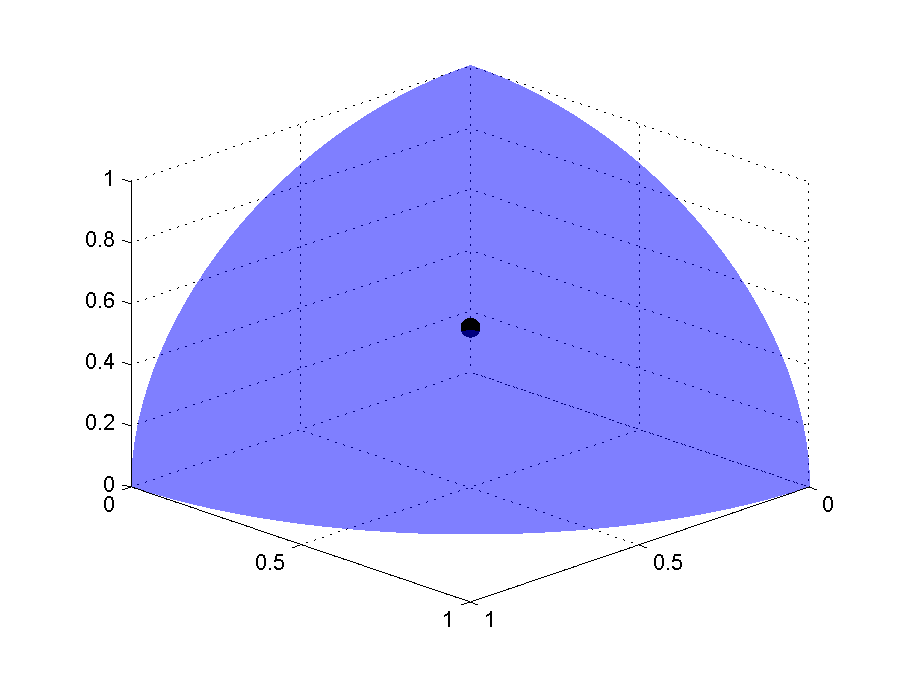
\includegraphics[width=0.92\textwidth]{figures/sec_Sn/LS2_3D.eps}
		\caption{}
	\end{subfigure}
	\hfill
	\begin{subfigure}[b]{0.48\textwidth}
		\centering
		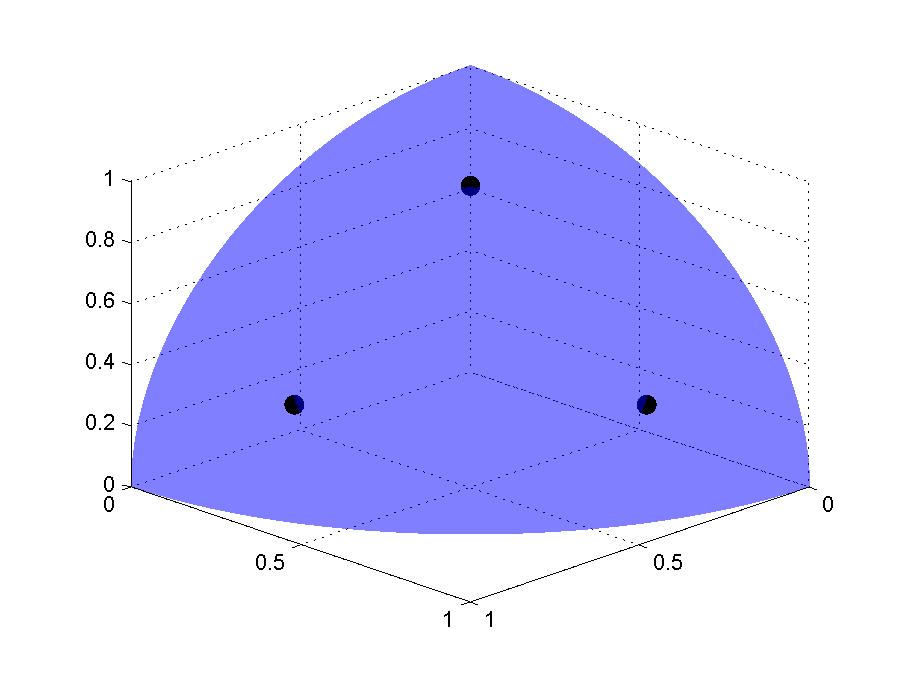
\includegraphics[width=0.92\textwidth]{figures/sec_Sn/LS4_3D.eps}
		\caption{}
	\end{subfigure}
	\vfill
	\begin{subfigure}[b]{0.48\textwidth}
		\centering
		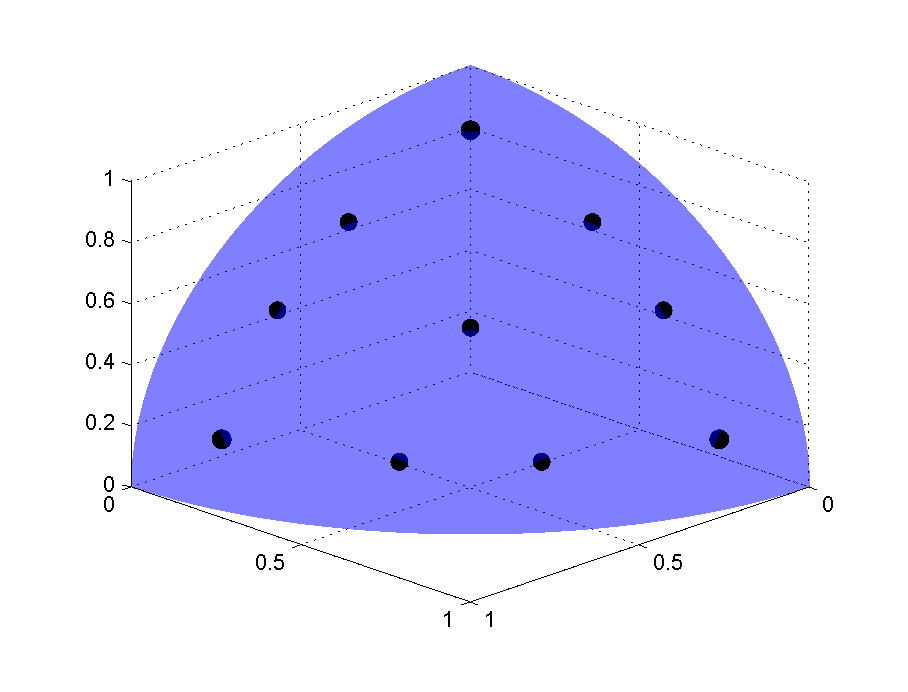
\includegraphics[width=0.92\textwidth]{figures/sec_Sn/LS8_3D.eps}
		\caption{}
	\end{subfigure}
	\hfill
	\begin{subfigure}[b]{0.48\textwidth}
		\centering
		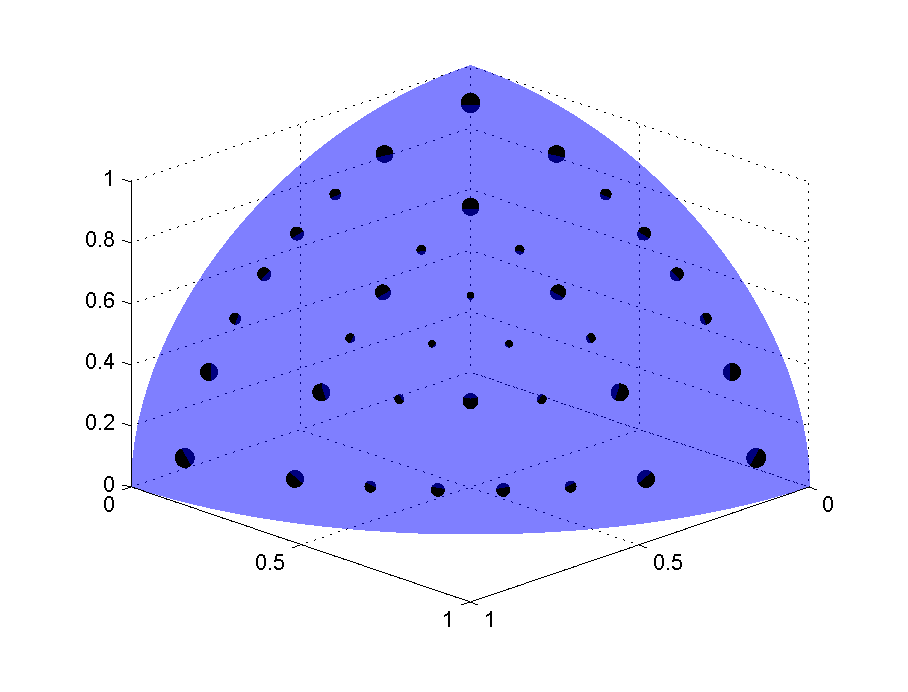
\includegraphics[width=0.92\textwidth]{figures/sec_Sn/LS16_3D.eps}
		\caption{}
	\end{subfigure}
\caption{Level-Symmetric angular quadrature sets of order (a) 2, (b) 4, (c) 8, and (d) 16.}
\label{fig::Sn_Angle_LS_Quads_3D}
\end{figure}

\begin{figure}
\centering
	\begin{subfigure}[b]{0.48\textwidth}
		\centering
		\includegraphics[width=0.92\textwidth]{figures/sec_Sn/LS2_2D.eps}
		\caption{}
	\end{subfigure}
	\hfill
	\begin{subfigure}[b]{0.48\textwidth}
		\centering
		\includegraphics[width=0.92\textwidth]{figures/sec_Sn/LS4_2D.eps}
		\caption{}
	\end{subfigure}
	\vfill
	\begin{subfigure}[b]{0.48\textwidth}
		\centering
		\includegraphics[width=0.92\textwidth]{figures/sec_Sn/LS8_2D.eps}
		\caption{}
	\end{subfigure}
	\hfill
	\begin{subfigure}[b]{0.48\textwidth}
		\centering
		\includegraphics[width=0.92\textwidth]{figures/sec_Sn/LS16_2D.eps}
		\caption{}
	\end{subfigure}
\caption{Projection of the 3D Level-Symmetric angular quadrature set with orders (a) 2, (b) 4, (c) 8, and (d) 16 onto the x-y space on the unit circle.}
\label{fig::Sn_Angle_LS_Quads_2D}
\end{figure}

%%%%%%%%%%%%%%%%%%%%%%%%%%%%%%%%%%%%%%%%%%%%%%%%%%%
%%%   SubSection - PGLC
\subsection{Product Gauss-Legendre-Chebyshev Quadrature Set}
\label{sec::Sn_Angle_PGLC}

The second angular quadrature set we will present is a Product Gauss-Legendre-Chebyshev (PGLC) set \cite{abu1977compatible}. It is formed by the product-wise multiplication of a Gauss-Chebyshev quadrature in the azimuthal direction and a Gauss-Legendre quadrature in the polar direction. It has the following key differences from the Level Symmetric set:

\begin{itemize}
	\item Does not have $90^o$ rotational invariance within the primary octant; however, we still maintain octant-to-octant symmetry via mapping;
	\item Has more control over the placement of the angular directions within the primary octant;
	\item Quadrature weights are aligned with the polar level;
	\item Has strictly positive weights for all polar and azimuthal combinations;
	\item Integrates exactly many of the spherical harmonics functions.
\end{itemize}

From the listed differences, we can already discern some clear advantages and disadvantages from a fully-symmetric quadrature set like LS. If a high number of angles are required for a problem, then negative weights do not arise. This is beneficial for transport problems with significant discontinuities. Also, the quadrature directions can be preferentially distributed in the primary octant if required for a particular problem. For example, if the transport solution is smoothly varying in the polar direction and not in the azimuthal direction, then we can specify a larger number of quadrature points in the azimuthal direction, with much fewer points in the polar direction. However, this also highlights the fact that the quadrature weights are aligned with the polar level, which can lead to less accurate moment integrations for certain transport problems. 

Because the PGLC quadrature set is formed by product-wise multiplication, we simply need to specify the component nodes and weights in both the azimuthal and polar directions to fully define all ordinates in the primary octant. The azimuthal direction, $\theta$, uses the positive range of the Gauss-Chebyshev quadrature set \cite{abramowitz1966handbook}. With the azimuthal direction restricted to its positive values in the primary octant, this corresponds to the upper-right portion of the unit circle: $\theta \in [0, \pi / 2]$. If we specify $A$ azimuthal directions for our quadrature set in the primary octant, then the azimuthal nodes and weights can be directly stated as 

\begin{equation}
\label{eq::Sn_Angle_GC_quad}
\theta_m = \frac{2m - 1}{4A} \pi \qquad \text{and} \qquad w_m = \frac{\pi}{2 A} ,
\end{equation}

\noindent respectively. 

For the polar direction, a Gauss-Legendre quadrature set is used \cite{abramowitz1964handbook}. Similar to the azimuthal direction, we restrict the integration of the polar direction to its positive values: $\xi \in (0,1)$. If we specify $P$ polar directions, then the cosines of the polar nodes, $\xi$, of our quadrature set are the positive roots of the $2P$-order Legendre polynomials taken over the interval $[-1, 1]$. In this case, we simply discard the negative roots. The corresponding Legendre weights are given by the following formula,

\begin{equation}
\label{eq::Sn_Angle_PGLC_legendre_weights}
w_n = \frac{2}{(1-\xi_n^2) (L_{2P}' (\xi_n))^2} ,
\end{equation}

\noindent where $ L_{2P}'$ is the derivative of the $2P$-order Legendre polynomial.

With the azimuthal directions specified by Eq. (\ref{eq::Sn_Angle_GC_quad}) and the polar cosines specified by the Legendre polynomial roots, any ordinate can now be determined by the definition of the angular directions in Eq. (\ref{eq::Sn_Angle_angle_components}). The ordinate weights can be specified in a similar manner. From Eqs. (\ref{eq::Sn_Angle_GC_quad}) and (\ref{eq::Sn_Angle_PGLC_legendre_weights}), any ordinate weight, $w_{m,n}$, can be calculated by the pairwise products of the azimuthal and polar weights: $w_{m,n} = w_m w_n$. This means that we can specify the integral, $F$, of some function $f (\theta, \gamma)$ over the primary octant of the unit sphere,

\begin{equation}
\label{eq::Sn_Angle_PGLC_product_weights}
F = \sum_{m=1}^{A} \sum_{n=1}^{P} w_m w_n  f(\theta_m , \gamma_n).
\end{equation}

For this dissertation, we will use the following notation to define the product nature of the PGLC quadrature points: $S_{A}^{P}$. Here, $A$ and $P$ correspond to the number of azimuthal and polar directions in the primary octant, respectively. We demonstrate this definition in Figure \ref{fig::Sn_Angle_PGLC_Quads_3D} for the primary octant with several combinations of azimuthal and polar directions. Figure \ref{fig::Sn_Angle_PGLC_Quads_2D} then presents the projections of these quadrature sets onto the unit circle for use in 2D transport problems. Again, the size of the direction marker corresponds to the relative weight of the quadrature point. One can clearly see that the weights vary on the polar levels, and all azimuthal weights on a given polar level are constant.

\begin{figure}
\centering
	\begin{subfigure}[b]{0.48\textwidth}
		\centering
		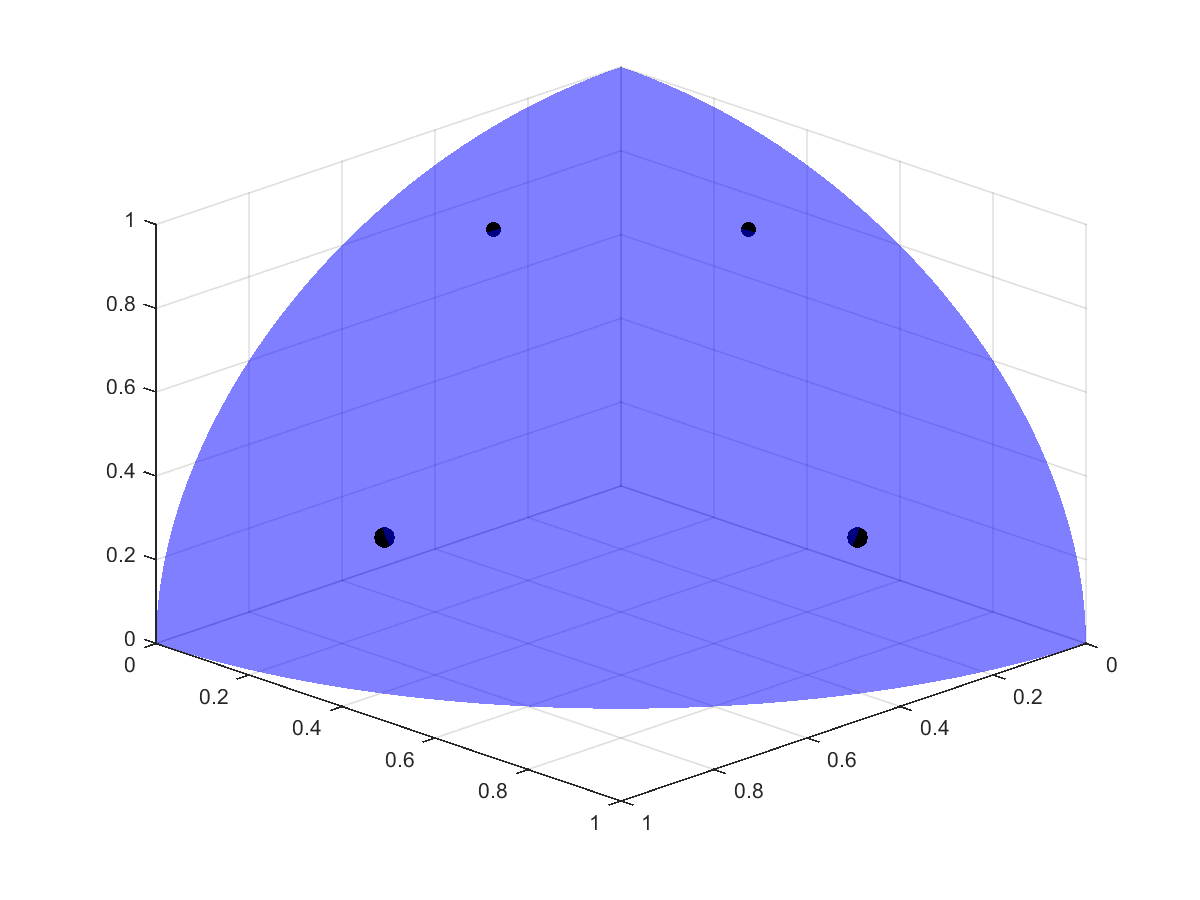
\includegraphics[width=0.92\textwidth]{figures/sec_Sn/PGLC2_2_3D.png}
		\caption{}
	\end{subfigure}
	\hfill
	\begin{subfigure}[b]{0.48\textwidth}
		\centering
		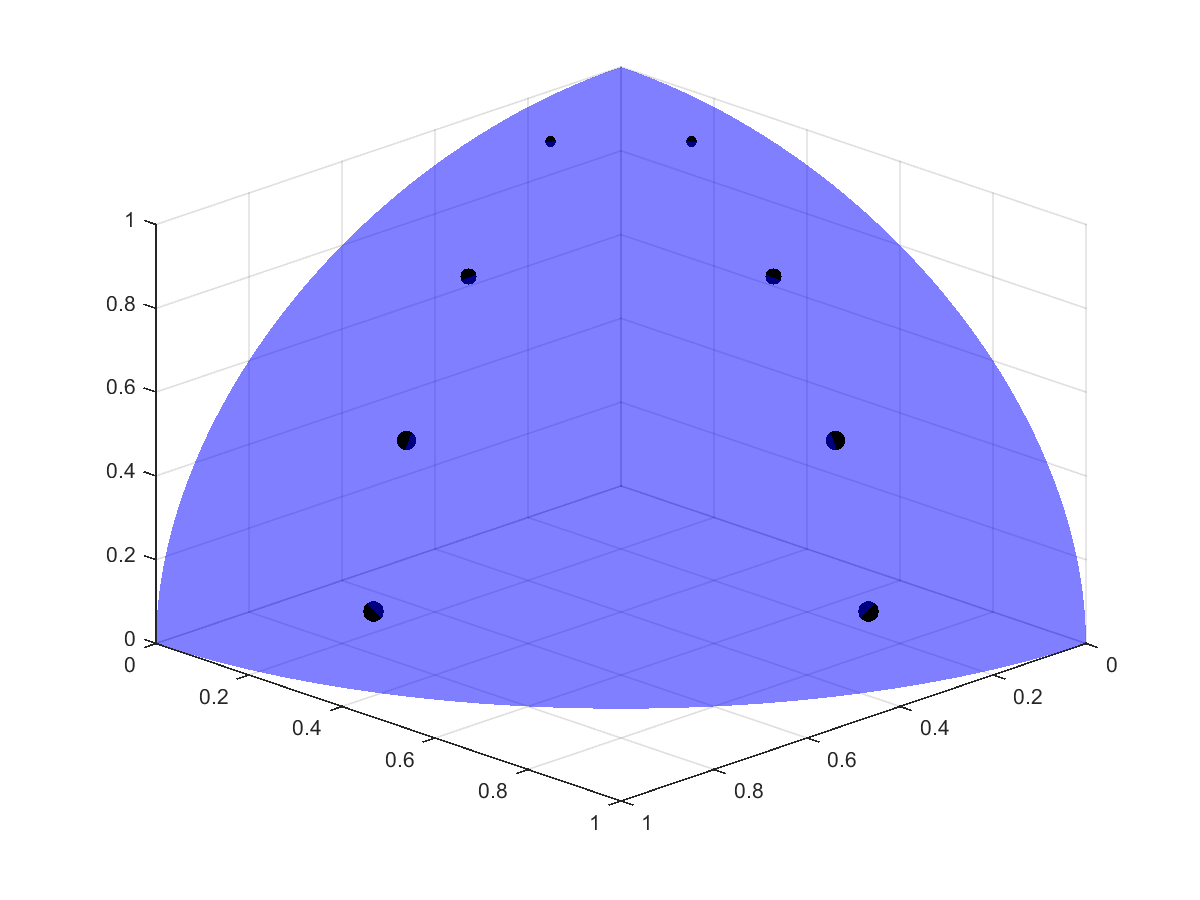
\includegraphics[width=0.92\textwidth]{figures/sec_Sn/PGLC2_4_3D.png}
		\caption{}
	\end{subfigure}
	\vfill
	\begin{subfigure}[b]{0.48\textwidth}
		\centering
		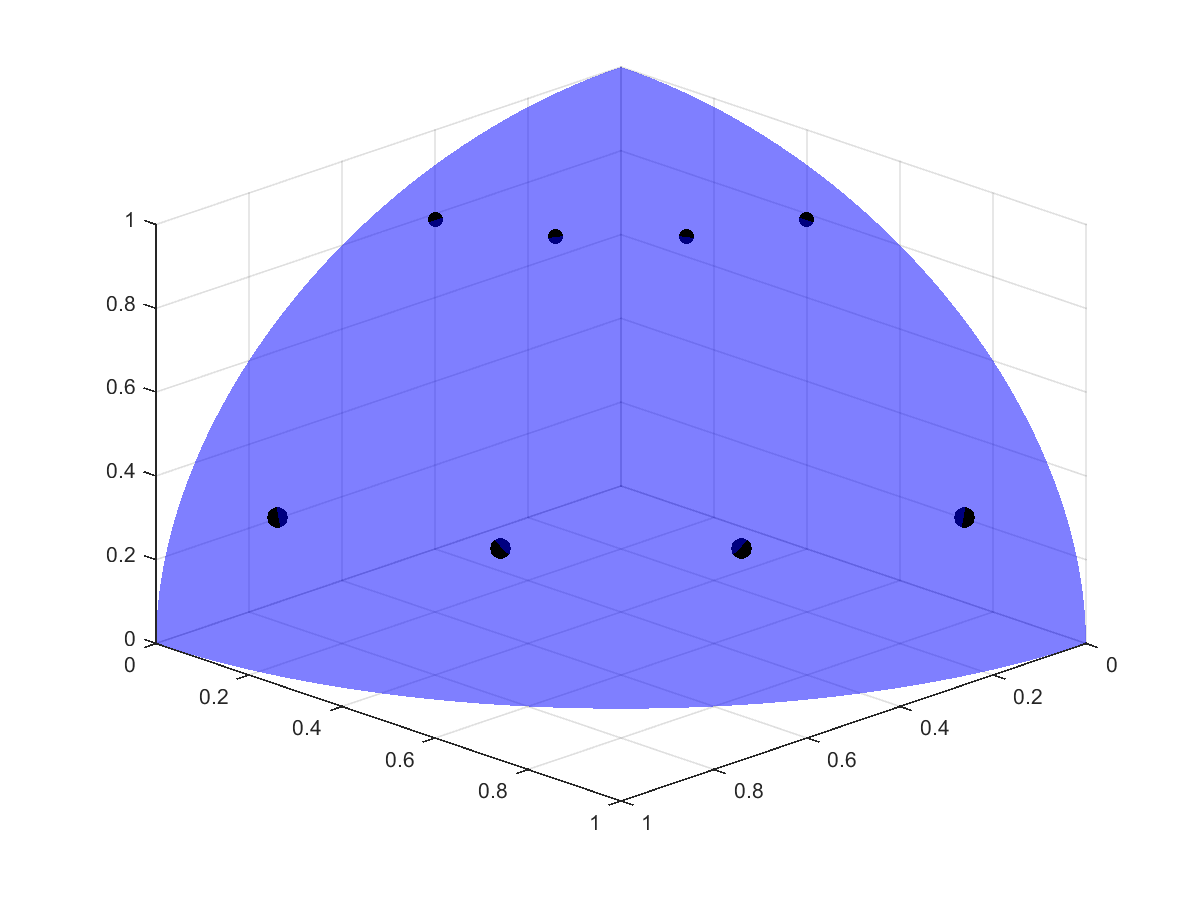
\includegraphics[width=0.92\textwidth]{figures/sec_Sn/PGLC4_2_3D.png}
		\caption{}
	\end{subfigure}
	\hfill
	\begin{subfigure}[b]{0.48\textwidth}
		\centering
		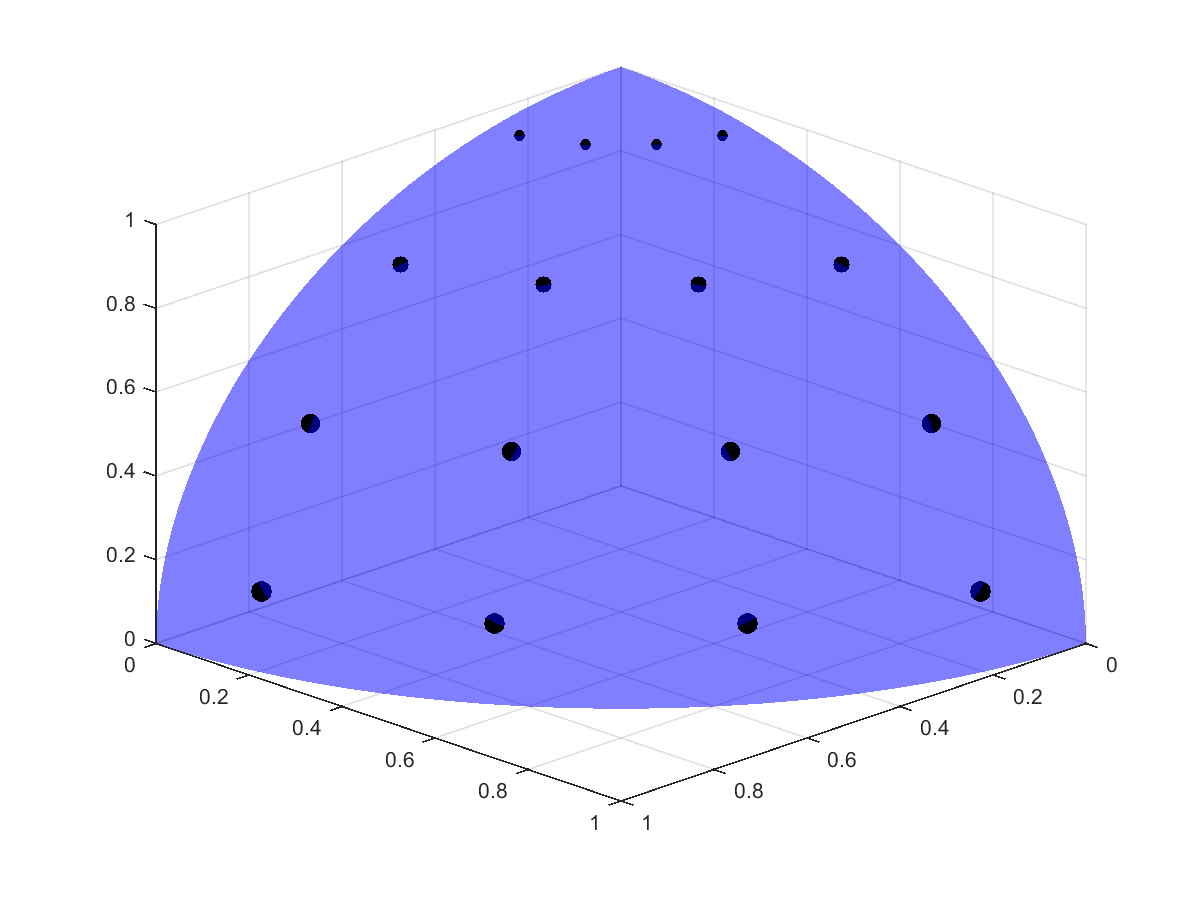
\includegraphics[width=0.92\textwidth]{figures/sec_Sn/PGLC4_4_3D.png}
		\caption{}
	\end{subfigure}
	\vfill
	\begin{subfigure}[b]{0.48\textwidth}
		\centering
		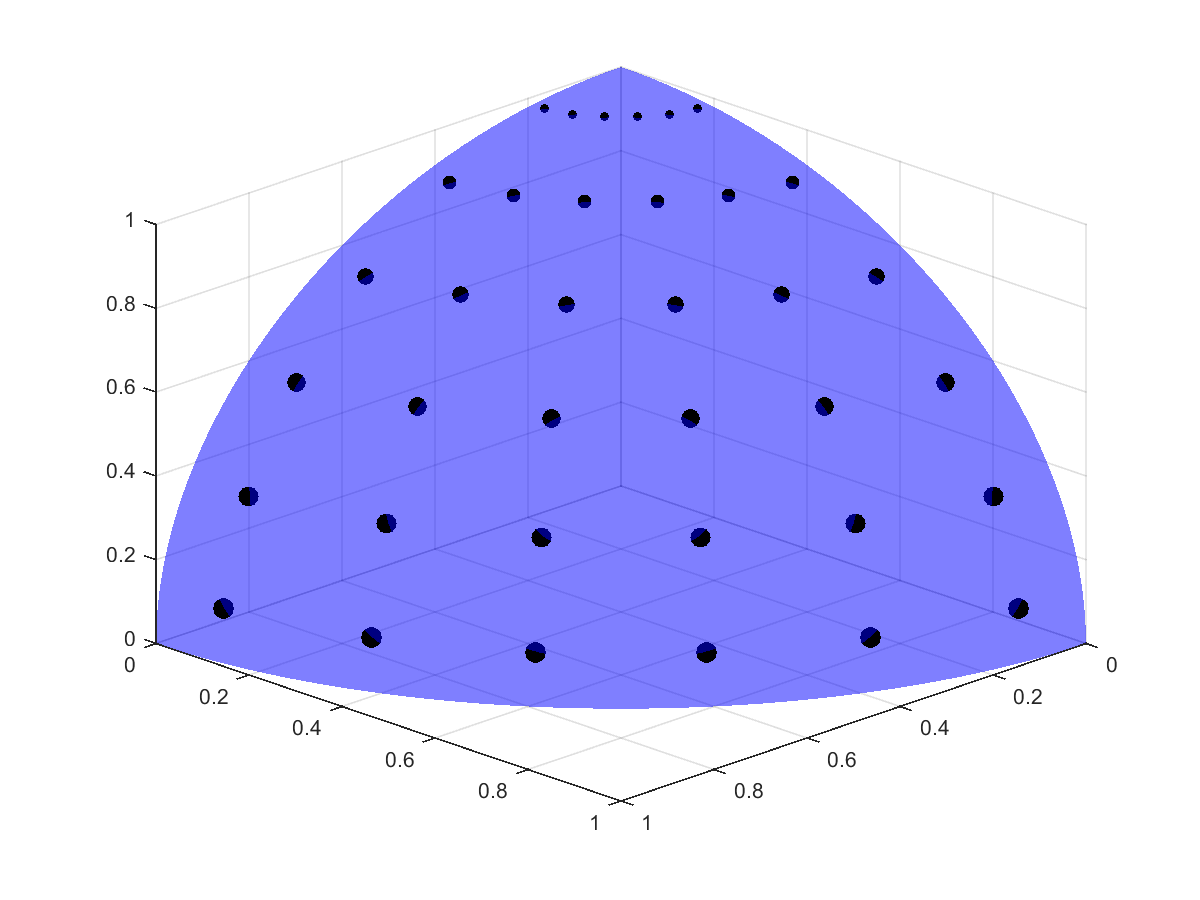
\includegraphics[width=0.92\textwidth]{figures/sec_Sn/PGLC6_6_3D.png}
		\caption{}
	\end{subfigure}
	\hfill
	\begin{subfigure}[b]{0.48\textwidth}
		\centering
		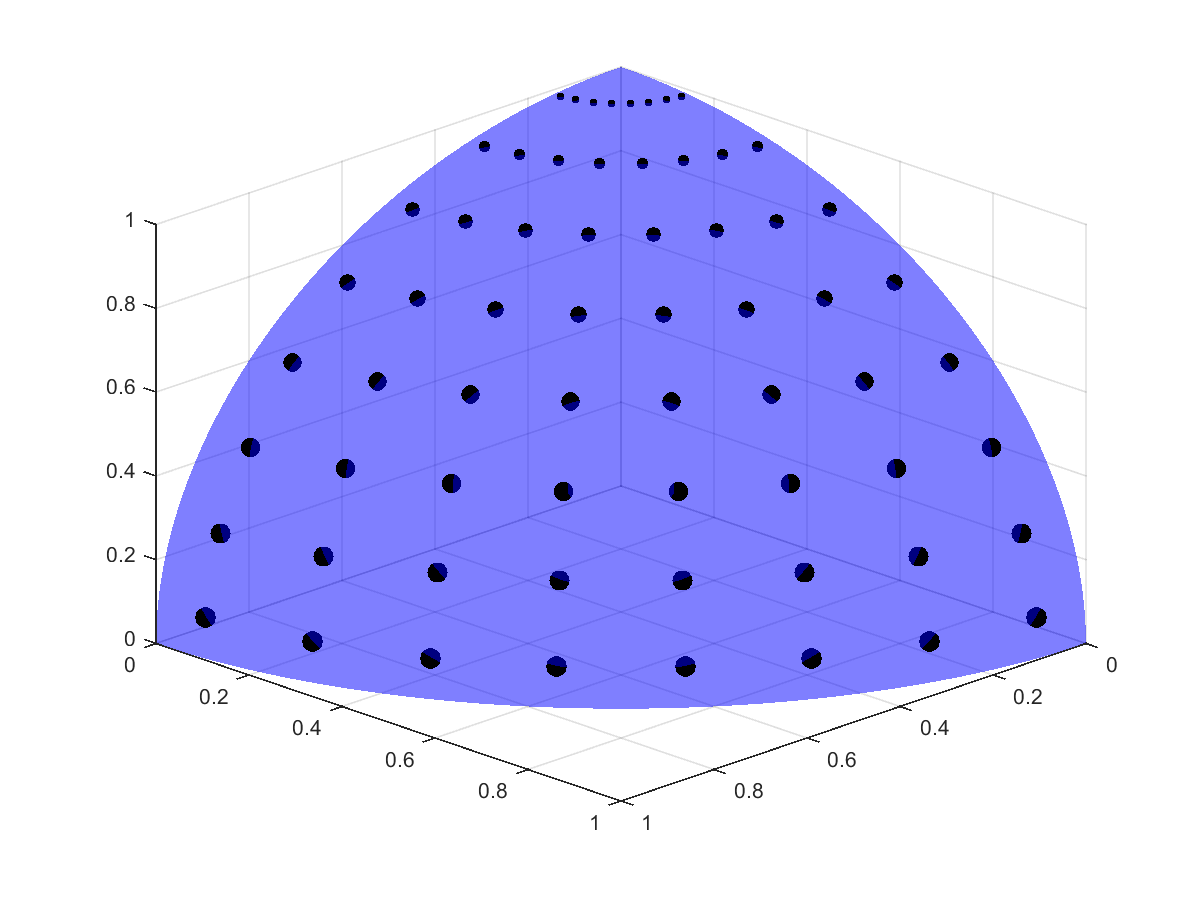
\includegraphics[width=0.92\textwidth]{figures/sec_Sn/PGLC8_8_3D.png}
		\caption{}
	\end{subfigure}
\caption{Product Gauss-Legendre-Chebyshev angular quadrature set with orders: (a) S$_2^2$, (b) S$_2^4$, (c) S$_4^2$, (d) S$_4^4$, (e) S$_6^6$, and (f) S$_8^8$.}
\label{fig::Sn_Angle_PGLC_Quads_3D}
\end{figure}

\begin{figure}
\centering
	\begin{subfigure}[b]{0.46\textwidth}
		\centering
		\includegraphics[width=0.85\textwidth]{figures/sec_Sn/PGLC2_2_2D.eps}
		\caption{}
	\end{subfigure}
	\hfill
	\begin{subfigure}[b]{0.46\textwidth}
		\centering
		\includegraphics[width=0.85\textwidth]{figures/sec_Sn/PGLC2_4_2D.eps}
		\caption{}
	\end{subfigure}
	\vfill
	\begin{subfigure}[b]{0.46\textwidth}
		\centering
		\includegraphics[width=0.85\textwidth]{figures/sec_Sn/PGLC4_2_2D.eps}
		\caption{}
	\end{subfigure}
	\hfill
	\begin{subfigure}[b]{0.46\textwidth}
		\centering
		\includegraphics[width=0.85\textwidth]{figures/sec_Sn/PGLC4_4_2D.eps}
		\caption{}
	\end{subfigure}
	\vfill
	\begin{subfigure}[b]{0.46\textwidth}
		\centering
		\includegraphics[width=0.85\textwidth]{figures/sec_Sn/PGLC6_6_2D.eps}
		\caption{}
	\end{subfigure}
	\hfill
	\begin{subfigure}[b]{0.46\textwidth}
		\centering
		\includegraphics[width=0.85\textwidth]{figures/sec_Sn/PGLC8_8_2D.eps}
		\caption{}
	\end{subfigure}
\caption{Projection of the 3D Product Gauss-Legendre-Chebyshev angular quadrature set with orders: (a) S$_2^2$, (b) S$_2^4$, (c) S$_4^2$, (d) S$_4^4$, (e) S$_6^6$, and (f) S$_8^8$ onto the x-y space on the unit circle.}
\label{fig::Sn_Angle_PGLC_Quads_2D}
\end{figure}

%%%%%%%%%%%%%%%%%%%%%%%%%%%%%%%%%%%%%%%%%%%%%%%%%%%
%%%   Section - Boundary Conditions
\section{Boundary Conditions}
\label{sec::Sn_BC}

Using the energy and angular discretizations presented in Sections \ref{sec::Sn_MG} and \ref{sec::Sn_Angle}, respectively, we write the standard, steady-state, multigroup $S_N$ transport equation for one angular direction, $m$, and one energy group, $g$:

\begin{equation}
\label{eq::Sn_mg_sn_trans_eq}
\begin{aligned}
	 \left( \vec{\Omega}_m \cdot \vec{\nabla}  + \sigma_{t,g}  \right)  \Psi_{m,g}= \sum_{g'=1}^{G} \sum_{p=0}^{N_P} \frac{2p + 1}{4 \pi} \sigma_{s,p}^{g' \rightarrow g}   \sum_{n=-p}^{p}  \Phi_{p,n,g'}  Y_{p,n} (  \vec{\Omega}_m )  \\
	+ \frac{\chi_g}{4 \pi} \sum_{g'=1}^{G} \nu \sigma_{f,g'} \Phi_{g'}   + Q_{m,g}
\end{aligned} , 
\end{equation}

\noindent where we have dropped the spatial parameter for clarity and is beholden to the following general, discretized boundary condition:

\begin{equation}
\label{eq::Sn_mg_sn_trans_eq_bc}
\Psi_{m,g} (\vec{r}) = \Psi^{inc}_{m,g} (\vec{r}) + \sum_{g'=1}^{G} \sum_{\vec{\Omega}_{m'} \cdot \vec{n} > 0} \gamma_{g' \rightarrow g}^{m' \rightarrow m} (\vec{r})  \Psi_{m',g'} (\vec{r})  .
\end{equation}

\noindent These $(M \text{x} G)$ discrete, tightly-coupled equations are currently defined as continuous in space.

For this dissertation work, we will consider only one type of boundary conditions: Dirichlet-type boundaries (also called {\em first-type boundary condition} in some physics and mathematical communities). In particular, we will only utilize incoming-incident and reflecting boundary conditions which correspond to $\vec{r} \in \partial \mathcal{D}^d$ and $\vec{r} \in \partial \mathcal{D}^r$, respectively. The full domain boundary is then the union: $\partial \mathcal{D} = \partial \mathcal{D}^d \cup \partial \mathcal{D}^r$. This leads to the boundary condition being succinctly written for one angular direction, $m$, and one energy group, $g$ as

\begin{equation}
\label{eq::Sn_simple_BC}
\Psi_{m,g} (\vec{r}) = \begin{cases}
	\Psi^{inc}_{m,g} (\vec{r}) , & \vec{r} \in \partial \mathcal{D}^d \\
	\Psi_{m',g} (\vec{r}) , & \vec{r} \in \partial \mathcal{D}^r
\end{cases}
\end{equation}

\noindent where the reflecting angle is $\vec{\Omega}_{m'} = \vec{\Omega}_{m} - 2 \left(  \vec{\Omega}_{m} \cdot \vec{n} \right) \vec{n}$ and $\vec{n}$ is oriented outward from the domain. To properly utilize the reflecting boundary condition that we have proposed, the angular quadrature set defined in Section \ref{sec::Sn_Angle} needs the following properties:

\begin{enumerate}
 	\item The reflected directions, $\vec{\Omega}_{m'}$, are also in the quadrature set for all $\vec{r} \in \partial \mathcal{D}^r$.
	\item The weights of the incident, $w_m$, and reflected, $w_{m'}$, angles must be equal.
\end{enumerate} 

\noindent For problems where the reflecting boundaries align with the $x,y,z$ axes, this will not be an issue with standard quadrature sets ({\em e.g.,} level-symmetric or Gauss-Legendre-Chebyshev). However, if the reflecting boundaries do not align in this manner, then additional care must be employed in calculating appropriate angular quadrature sets.

%%%%%%%%%%%%%%%%%%%%%%%%%%%%%%%%%%%%%%%%%%%%%%%%%%%
%%%   Section - Spatial Discretization
\section{Spatial Discretization}
\label{sec::Sn_Spatial}

For the spatial discretization of the problem domain, we simplify Eq. (\ref{eq::Sn_mg_sn_trans_eq}) into a single energy group and drop the fission term (it can be lumped into the 0th moment of the source term and will act similarly to the total interaction term)

\begin{equation}
\label{eq::Sn_trans_eq_simple_no_energy_groups}
\vec{\Omega}_m \cdot \vec{\nabla} \Psi_{m}  + \sigma_{t}   \Psi_{m}=  \sum_{p=0}^{N_P} \frac{2p + 1}{4 \pi}    \sum_{n=-p}^{p}  Y_{p,n} (  \vec{\Omega}_m ) \left[ \sigma_{s,p}  \Phi_{p,n,}  + Q_{p,n} \right]
\end{equation}

\noindent to form $M$ ($m=1,...,M$) angularly discrete equations. We then lay down an unstructured mesh, $\mathbb{T}_h \in \mathbb{R}^{d}$, over the spatial domain, where $d$ is the dimensionality of the problem ($d=1,2,3$). This mesh consists of non-overlapping spatial elements to form a complete union over the entire spatial domain: $\mathcal{D} = \bigcup_{K \in \mathbb{T}_h} K$. To form the DGFEM set of equations \cite{ern2013theory,wareing2001discontinuous}, we consider a spatial cell $K \in \mathbb{R}^d$ which has $N_V^K$ vertices and $N_f^K$ faces. Each face of cell $K$ resides in dimension $\mathbb{R}^{d-1}$ and is formed by a connection of a subset of vertices. For a 1D problem, each face is a single point. For a 2D problem, each face is a line segment connecting two distinct points. For a 3D problem, each face is a $\mathbb{R}^2$ closed polygon (not necessarily coplanar) which may or may not be convex. An example of this interconnection between elements is given for a $\mathbb{R}^2$ problem in Figure \ref{fig::Sn_two_ref_cells} between our cell of interest, $K$, and another cell, $K'$, separated by the face $f$. We have chosen the normal direction of the face to have orientation from cell $K$ to cell $K'$ while we form the DGFEM equations for cell $K$. This means that if we were instead analyzing cell $K'$, then the face $f$ normal, $\vec{n}' $, would be opposite ({\em i.e.,} $\vec{n}' = -\vec{n}$).

\begin{figure}
\centering
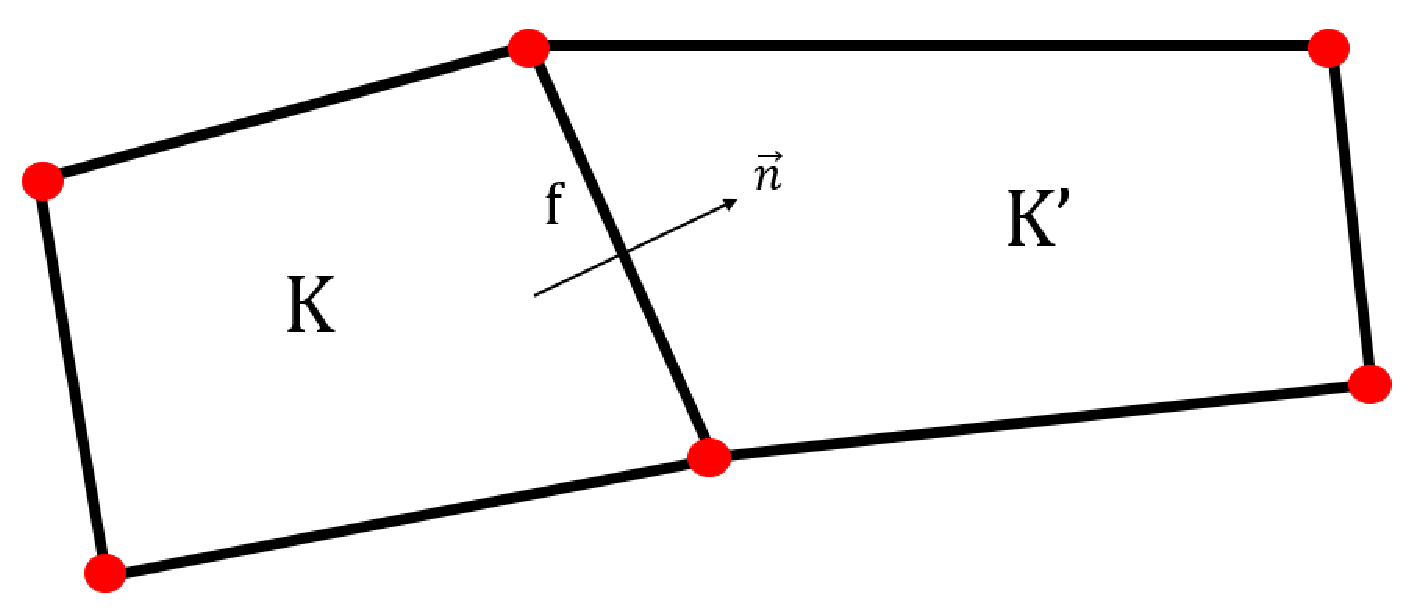
\includegraphics[width=0.7\textwidth]{figures/sec_Sn/two_cells_Rev1.eps}
\caption{Two cells of the spatial discretization with the connecting face, $f$, with normal direction, $\vec{n}$, oriented from cell $K$ to cell $K'$.}
\label{fig::Sn_two_ref_cells}
\end{figure}

Next, we multiply Eq. (\ref{eq::Sn_trans_eq_simple_no_energy_groups}) by an appropriate test function $b_m$, integrate over cell $K$, and apply Gauss' Divergence Theorem to the streaming term to obtain the Galerkin weighted-residual for cell $K$ for an angular direction $\vec{\Omega}_m$:

\begin{equation}
\label{eq::Sn_DGFEM_trans_eq_cellK}
\begin{aligned}
- \left( \vec{\Omega}_m \cdot  \vec{\nabla} b_m, \Psi_{m} \right)_{K} + \sum_{f=1}^{N_f^K} \Big< ( \vec{\Omega}_m \cdot \vec{n} ) \, b_m, \tilde{\Psi}_m  \Big>_{f}  + \Big(  \sigma_{t} b_m ,   \Psi_{m} \Big)_{K} \\
= \sum_{p=0}^{N_P} \sum_{n=-p}^{p} \frac{2p + 1}{4 \pi}  Y_{p,n} (  \vec{\Omega}_m ) \left[ \Big( \sigma_{s,p} \, b_m,  \Phi_{p,n,} \Big)_{K}  + \left(  b_m ,   Q_{p,n} \right)_{K} \right]
\end{aligned} .
\end{equation}

\noindent The cell boundary fluxes, $\tilde{\Psi}_m$, will depend on the cell boundary type and will be defined shortly. The cell boundary $\partial \mathcal{D}_K = \bigcup_{ f \in N_f^K} f$ is the closed set of the $N_f^K$ faces of the geometric cell. The inner products:

\begin{equation}
\label{eq::Sn_spatial_inner_products_cell}
 \Big( u, v \Big)_K \equiv \int_K u \, v \, d r
\end{equation} 

\noindent and

\begin{equation}
\label{eq::Sn_spatial_inner_products_face}
 \Big< u, v \Big>_f \equiv \int_f u \, v \, d s
\end{equation}

\noindent correspond to integrations over the cell volume and faces, respectively, where $dr \in \mathbb{R}^d$ is within the cell and $ds \in \mathbb{R}^{d-1}$ is along the cell boundary. We note that we will use this notation of the inner product for the remainder of the dissertation unless otherwise stated. We then separate the summation of the cell $K$ boundary integration terms into two different types: outflow boundaries ($\partial K^+ = \{  \vec{r} \in \partial K: \vec{n} (\vec{r}) \cdot \vec{\Omega}_m > 0 \}$) and inflow boundaries ($\partial K^- = \{  \vec{r} \in \partial K: \vec{n} (\vec{r}) \cdot \vec{\Omega}_m < 0 \}$). The inflow boundaries can further be separated into inflow from another cell: $\partial K^- \backslash \partial \mathcal{D} $; inflow from incident flux on the domain boundary: $\partial K^- \cap \partial \mathcal{D}^d $; and reflecting domain boundaries: $\partial K^- \cap \partial \mathcal{D}^r $. At this point, we note that the derivation can comprise an additional step by using Gauss' Divergence Theorem again on the streaming term. This is sometimes performed for radiation transport work so that mass matrix lumping can be performed, but we will not do so here at this time. Therefore, with the cell boundary terminology as proposed, Eq. (\ref{eq::Sn_DGFEM_trans_eq_cellK}) can be written into the following form:

\begin{equation}
\label{eq::Sn_DGFEM_trans_eq_cellK_diff_faces}
\begin{aligned}
&- \left( \vec{\Omega}_m \cdot  \vec{\nabla} b_m, \Psi_{m} \right)_{K}   + \Big(  \sigma_{t} b_m ,   \Psi_{m} \Big)_{K}  \\
&+  \Big< ( \vec{\Omega}_m \cdot \vec{n} ) \, b_m, \tilde{\Psi}_m  \Big>_{\partial K^+}  + \Big< ( \vec{\Omega}_m \cdot \vec{n} ) \, b_m, \tilde{\Psi}_m  \Big>_{\partial K^- \backslash \partial \mathcal{D}} \\
  &+ \Big< ( \vec{\Omega}_m \cdot \vec{n} ) \, b_m, \tilde{\Psi}_m  \Big>_{\partial K^- \cap \partial \mathcal{D}^d}  + \Big< ( \vec{\Omega}_m \cdot \vec{n} ) \, b_m, \tilde{\Psi}_m  \Big>_{\partial K^- \cap \partial \mathcal{D}^r}  \\
&= \sum_{p=0}^{N_P} \sum_{n=-p}^{p} \frac{2p + 1}{4 \pi}  Y_{p,n} (  \vec{\Omega}_m ) \left[ \Big( \sigma_{s,p} \, b_m,  \Phi_{p,n,} \Big)_{K}  + \left(  b_m ,   Q_{p,n} \right)_{K} \right]
\end{aligned} .
\end{equation}

We can now deal with the boundary fluxes, $\tilde{\Psi}_m$, by enforcing the ubiquitously-used {\em upwind scheme}. In simple nomenclature, the upwind scheme corresponds to using the angular flux values within the cell for outflow boundaries and angular flux values outside the cell for inflow boundaries. Mathematically, the upwind scheme can succinctly be written as the following for all boundary types,

\begin{equation}
\label{eq::Sn_upwind_cases}
\tilde{\Psi}_m (\vec{r}) = \begin{cases}
\Psi_m^{-} , & \partial K^+ \\
\Psi_m^{-}, & \partial K^- \backslash \partial \mathcal{D} \\
\Psi_m^{inc}, & \partial K^- \cap \partial \mathcal{D}^d \\
\Psi_{m'}^{-}, & \partial K^- \cap \partial \mathcal{D}^r
\end{cases} ,
\end{equation}

\noindent when the following trace is applied to the angular fluxes :

\begin{equation}
\label{eq::Sn_ang_flux_trace}
\Psi_m^{\pm} (\vec{r}) \equiv \lim_{s \rightarrow 0^{\pm}} \Psi_m \Big( \vec{r} + s (\vec{\Omega}_m \cdot \vec{n}) \vec{n} \Big) .
\end{equation}

\begin{figure}
\centering
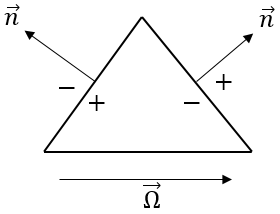
\includegraphics[width=0.35\textwidth]{figures/sec_Sn/upwind_triangle.png}
\caption{Definition of the trace for the upwinding scheme.}
\label{fig::Sn_Spatial_upwind_triangle}
\end{figure}

\noindent We give a visual example of this trace in Figure \ref{fig::Sn_Spatial_upwind_triangle} on a triangle with a single inflow and a single outflow boundary. For the inflow (left) boundary, the within-cell fluxes are ``+'' and the out-of-cell fluxes are ``-''. Likewise, the outflow (right) boundary has within-cell fluxes designated as ``-'' and out-of-cell fluxes designated as ``+''. Therefore, with this definition of the trace, we always use the flux values corresponding to the ``-'' direction (as seen in Eq. (\ref{eq::Sn_upwind_cases})). Now, using the upwind scheme as previously defined, we can write our complete set of DGFEM equations for cell $K$ as

\begin{equation}
\label{eq::Sn_DGFEM_trans_eq_cellK_complete}
\begin{aligned}
-  \Big( \vec{\Omega}_m \cdot  & \vec{\nabla} b_m, \Psi_{m} \Big)_{K}   + \Big(  \sigma_{t} b_m ,   \Psi_{m} \Big)_{K} +  \Big< ( \vec{\Omega}_m \cdot \vec{n} ) \, b_m, {\Psi}_m^{-}  \Big>_{\partial K^+}  \\
  + & \Big< ( \vec{\Omega}_m \cdot \vec{n} ) \, b_m, {\Psi}_m^{-}  \Big>_{\partial K^- \backslash \partial \mathcal{D}}  + \Big< ( \vec{\Omega}_m \cdot \vec{n} ) \, b_m, {\Psi}^{-}_{m'}  \Big>_{\partial K^- \cap \partial \mathcal{D}^r}  \\
= & \sum_{p=0}^{N_P} \sum_{n=-p}^{p} \frac{2p + 1}{4 \pi}  Y_{p,n} (  \vec{\Omega}_m ) \left[ \Big( \sigma_{s,p} \, b_m,  \Phi_{p,n,} \Big)_{K}  + \left(  b_m ,   Q_{p,n} \right)_{K} \right] \\
- & \Big< ( \vec{\Omega}_m \cdot \vec{n} ) \, b_m, {\Psi}_m^{inc}  \Big>_{\partial K^- \cap \partial \mathcal{D}^d}
\end{aligned} .
\end{equation} 

\noindent We note that fluxes without the trace superscript are all within the cell. Also, the basis functions, $b_m$, always correspond to within the cell. By completely defining our mathematical formulation for an arbitrary spatial cell, it is easy to see that the full set of equations to define our discretized solution space for a single angle and energy group comprises of a simple double integration loop. The full set of equations can be formed by looping over all spatial cells, $\mathcal{D} = \bigcup_{K \in \mathbb{T}_h} K$, while further looping over all faces within each cell, $\partial \mathcal{D}_K = \bigcup_{ f \in N_f^K} f$. 

%%%%%%%%%%%%%%%%%%%%%%%%%%%%%%%%%%%%%%%%%%%%%%%%%%%
%%%   SubSection - Convergence
\subsection{Convergence Rates of the DGFEM $S_N$ Equation}
\label{sec::Sn_Spatial_Convergence}

Because we seek to investigate the use of high-order spatial basis functions for the transport equation, we need to form an estimate of the spatial error based on some measure of the mesh. We do this by taking Eq. (\ref{eq::Sn_DGFEM_trans_eq_cellK_complete}), performing another integration-by-parts on the streaming term, multiplying by the angular weight, $w_m$, and summing over all elements and all angular directions. We also change the notation of the test function from $b_m$ to $\Psi_m^{*}$ to ease notation at a later step. This leads to the variational form for the 1-group $S_N$ equation:

\begin{equation}
\label{eq::Sn_DGFEM_variational_form}
\begin{aligned}
\sum\displaylimits_{m=1}^M w_m& \Big[  \Big(  \Psi_m^*, \vec{\Omega}_m \cdot   \vec{\nabla} \Psi_{m} \Big)_{\mathcal{D}} + \Big( \sigma_t  \Psi_m^{*},  \Psi_{m} \Big)_{\mathcal{D}}  \Big]  \\
+ \sum\displaylimits_{m=1}^M w_m& \Big< ( \vec{\Omega}_m \cdot \vec{n} ) \, \Psi_m^{* +}, [\![ \Psi_m]\!]  \Big>_{E_h^i} \\
+ \sum\displaylimits_{m=1}^M w_m& \Big[ \Big< ( \vec{\Omega}_m \cdot \vec{n} ) \, \Psi_m^{*}, {\Psi}_{m'}  \Big>_{\partial \mathcal{D}_m^{r-}} -  \Big< ( \vec{\Omega}_m \cdot \vec{n} ) \, \Psi_m^{*}, {\Psi}_m  \Big>_{\partial \mathcal{D}_m^-}   \Big] \\
= \sum\displaylimits_{m=1}^M w_m&     \sum_{p=0}^{N_P} \sum_{n=-p}^{p} \frac{2p + 1}{4 \pi}  Y_{p,n} (  \vec{\Omega}_m )  \Big(   \Psi_m^{*}, \sigma_{s,p} \,  \Phi_{p,n,} +  Q_{p,n} \Big)_{\mathcal{D}}  \\
- \sum\displaylimits_{m=1}^M w_m&   \Big< ( \vec{\Omega}_m \cdot \vec{n} ) \, \Psi_m^{*}, {\Psi}_m^{inc}  \Big>_{\partial \mathcal{D}_m^- }
\end{aligned}
\end{equation}

\noindent where the inner products over the whole domain and over all interior faces are

\begin{equation}
\label{eq::Sn_DGFEM_vol_inner_prod}
\Big( u, v \Big)_{\mathcal{D}} \equiv \sum_{K \in \mathbb{T}_h}  \Big( u, v \Big)_{K} ,
\end{equation}

\noindent and 

\begin{equation}
\label{eq::Sn_DGFEM_surf_inner_prod}
\Big< u, v \Big>_{E_h^i} \equiv \sum_{f \in E_h^i}  \Big< u, v \Big>_{f} ,
\end{equation}

\noindent respectively. The interior faces are designated as the non-repeating set: $E_h^i \in \cup_{K \in  \mathbb{T}_h} \partial K \backslash \partial \mathcal{D}$. In Eq. (\ref{eq::Sn_DGFEM_variational_form}), the interior jump term, $[\![ \Psi_m]\!]$, is defined as,

\begin{equation}
\label{eq::Sn_Spatial_Convergence_jump}
[\![ \Psi_m]\!] = \Psi_m^{+} - \Psi_m^{-} ,
\end{equation}

\noindent and along with the inflow basis function, $b_m^{+}$, is beholden to the following trace condition:

\begin{equation}
\label{eq::Sn_Spatial_Convergence_trace}
\begin{aligned}
\Psi_m^{\pm} \equiv \lim\displaylimits_{s \rightarrow 0^\pm} \Psi_m (\vec{r} - u (\vec{r})  s  \, \vec{\Omega}_m ) \\
u (\vec{r}) = \text{sgn} \left(  \vec{n} (\vec{r}) \cdot  \vec{\Omega}_m \right)
\end{aligned} .
\end{equation}

We can give compact notation to the variational form of the DGFEM transport equation in Eq. (\ref{eq::Sn_DGFEM_variational_form}) by defining the bilinear form in Eq. (\ref{eq::Sn_Spatial_Convergence_bilinear}). We have changed the sequence of the summation over directions and over the elements for the boundary terms.

\begin{equation}
\label{eq::Sn_Spatial_Convergence_bilinear}
\begin{aligned}
a(\Psi^{*},\Psi) = \sum\displaylimits_{m=1}^M w_m \Big[  \Big(  \Psi_m^{*}, \vec{\Omega}_m \cdot   \vec{\nabla} \Psi_{m} \Big)_{\mathcal{D}} + \Big( \sigma_t  \Psi_m^{*},  \Psi_{m} \Big)_{\mathcal{D}}  \Big]  \\
+ \sum\displaylimits_{m=1}^M w_m \Big< ( \vec{\Omega}_m \cdot \vec{n} ) \, \Psi_m^{* +}, [\![ \Psi_m]\!]  \Big>_{E_h^i} - \sum\displaylimits_{f \in \partial \mathcal{D}} \sum\displaylimits_{\vec{\Omega}_m \cdot \vec{n}} \Big< ( \vec{\Omega}_m \cdot \vec{n} ) \, \Psi_m^{*}, {\Psi}_m  \Big>_{f}  \\
+ \sum\displaylimits_{f \in \partial \mathcal{D}^r} \sum\displaylimits_{\vec{\Omega}_m \cdot \vec{n}} \Big< ( \vec{\Omega}_m \cdot \vec{n} ) \, \Psi_m^{*}, {\Psi}_{m'}  \Big>_{f} -      \sum_{p=0}^{N_P} \sum_{n=-p}^{p} \frac{2p + 1}{4 \pi}   \Big(  \sigma_{s,p} \,  \Phi_{p,n,}^{*},  \Phi_{p,n,} \Big)_{\mathcal{D}} 
\end{aligned}
\end{equation}

\noindent This bilinear form is positive definite ($a(\Psi,\Psi) > 0$) but obviously not symmetric. It also holds Galerkin orthogonality, which means that the jumps across elements for the exact solution are zero,

\begin{equation}
\label{eq::Sn_Spatial_Convergence_Galerkin_orth}
a(\Psi^{*},\Psi - \Psi_{exact})  = 0, \qquad m=1,...,M .
\end{equation}

\noindent Because of the positive definiteness and Galerkin orthogonality of the bilinear form, we can use it to define a DG-norm,

\begin{equation}
\label{eq::Sn_Spatial_Convergence_DGnorm_bilinear}
|| u  ||_{DG} = a(u,u).
\end{equation}

\noindent We can also give a more simplified definition of the DG norm,

\begin{equation}
\label{eq::Sn_Spatial_Convergence_DGform}
|| u ||^2_{DG} = \sum_{K \in \mathbb{T}_h} \left[  || u  ||^2_{L^2 (K)} + \frac{1}{2} || u^+ - u^- ||_{L^2 (\partial K)} \right],
\end{equation}

\noindent which contains the standard $L_2$ norm in the element interiors as well as additional $L_2$ norms on the element boundaries corresponding to the jump terms across the mesh cells.

The convergence of DGFEM methods for the hyperbolic systems has been extensively studied \cite{lesaint1974finite,houston2000stabilized,houston2002discontinuous,wang2009convergence}. With the discretized flux solutions, $\Psi_h \in W^h_{\mathcal{D}}$ and $\Phi_h \in W^h_{\mathcal{D}}$, corresponding to our unstructured, $\mathbb{T}_h$, we can define an error for our DGFEM transport solution with the DG norm for the angular fluxes,


\begin{equation}
\label{eq::Sn_Spatial_Convergence_DGnorm_psi}
|| \Psi - \Psi_{exact} ||_{DG} \leq C \frac{h^q}{(p+1)^q},
\end{equation}

\noindent and flux moments,

\begin{equation}
\label{eq::Sn_Spatial_Convergence_DGnorm_phi}
|| \Phi - \Phi_{exact} ||_{DG} \leq C \frac{h^q}{(p+1)^q},
\end{equation}

\noindent respectively. In Eqs. (\ref{eq::Sn_Spatial_Convergence_DGnorm_psi}) and (\ref{eq::Sn_Spatial_Convergence_DGnorm_phi}), $q = \min (p+1/2, r - 1/2)$, $h$ is the maximum diameter of all the mesh elements, $p$ is the polynomial completeness of the finite element function space (this will be explained further in Chapter \ref{sec::BF}), $r$ is the regularity index of the transport solution, and $C$ is a constant that is independent of the mesh employed. We can also give an estimate for the transport solution error in the standard $L_2$ norm,

\begin{equation}
\label{eq::Sn_Spatial_Convergence_L2norm_phi}
|| \Phi - \Phi_{exact} ||_{L_2} \leq C \frac{h^{q+1/2}}{(p+1)^q},
\end{equation}

\noindent where $q$ has the same definition as before. We can see that for the $L_2$ norm the convergence rate is simply $1/2$ integer more than the DG norm for both the polynomial order and the regularity index.

Investigating the definition of the $q$ term in Eqs. (\ref{eq::Sn_Spatial_Convergence_DGnorm_psi}), (\ref{eq::Sn_Spatial_Convergence_DGnorm_phi}), and (\ref{eq::Sn_Spatial_Convergence_L2norm_phi}) further, we can see that our DGFEM transport convergence rates are all limited by the regularity, $r$, of the solution space. The spaces in which the transport equation can reside have been investigated by others in previous works \cite{wang2009convergence,magenes1970problemes,johnson1983convergence}. If we have sufficiently smooth data, then the exact transport solution belongs, at most, in the $H^{3/2-\epsilon} (\mathcal{D})$ Hilbert space. This yields a solution regularity of $r=\frac{3}{2}-\epsilon$, where $\epsilon$ is positive and extremely small. This means that, for most practical occurrences, the observed converge regularity is simply $\frac{3}{2}$. For this case, it is sufficient to have piecewise polynomial cross section data and incident boundary fluxes that align with our mesh. However, in the case of a pure absorber or void, the exact transport solution lives in the $H^{1/2-\epsilon} (\mathcal{D})$ Hilbert space. Again, the practical irregularity becomes $\frac{1}{2}$. From these spaces, one would think that the transport solution regularity would impede the use of higher-order finite element spaces. We note, however, that these regularity indices only apply to the asymptotic convergence range, which usually only applies to very fine meshes that are much smaller than typically employed meshes. Therefore, we expect to capture up to order $(p+1)$ convergence in preasymptotic ranges that would be employed for a wide variety of transport problems. Results capturing this irregularity behavior are presented in Chapter \ref{sec::BF}.

Finally, we also seek to define the transport solution convergence rates in terms other than the maximum element diameter, $h$. For polytope meshes, this metric may not be the easiest to compute or report if there is large variability in the polygonal or polyhedral elements of the mesh. We seek to re-express the convergence rates in terms of the total number of degrees of freedom in the problem, $N_{dof}$, instead of the maximum element diameter, $h$. First, we relate the total number of elements, $N_{ele}$, to the maximum element diameter,

\begin{equation}
\label{eq::Sn_Spatial_Convergence_Nele_to_h}
N_{ele} \propto h^{-d},
\end{equation}

\noindent where we assume that the polytope elements are convex and reasonably regular. We then assume that the finite element functional space on each element is the Serendipity space (we go into further detail in Chapter \ref{sec::BF}) \cite{macneal1992eight,arnold2011serendipity}. This means that the number of degrees of freedom per element is proportional to the polynomial order: $N_{dof} \propto p h^{-d}$ or $h \propto \left(  \frac{N_{dof}}{p} \right)^{-1/d}$. We substitute this result into Eq. (\ref{eq::Sn_Spatial_Convergence_L2norm_phi}) to yield an $L_2$ convergence rate in terms of the problem's total number of degrees of freedom,

\begin{equation}
\label{eq::Sn_Spatial_Convergence_L2norm_phi_Ndof}
|| \Phi - \Phi_{exact} ||_{L_2} \leq C (p) N_{dof}^{-\frac{q+1/2}{d}},
\end{equation}

\noindent where the proportionality constant, $C(p)$, now has the form,

\begin{equation}
\label{eq::Sn_Spatial_Convergence_Cconstant}
C(p) =  \frac{p^{\frac{q+1/2}{d}}}{(p+1)^q}.
\end{equation}

\noindent For a transport problem that is not bound by the solution regularity, we can express the simplified convergence rate,

\begin{equation}
\label{eq::Sn_Spatial_Convergence_L2norm_phi_Ndof_full}
|| \Phi - \Phi_{exact} ||_{L_2} \leq C(p) \, N_{dof}^{-\frac{p+1}{d}}, \qquad C(p) = \frac{p^{\frac{p+1}{d}}}{(p+1)^{p+1/2}}.
\end{equation}

\noindent The result of Eq. (\ref{eq::Sn_Spatial_Convergence_L2norm_phi_Ndof_full}) states that we expect convergence rates of $N_{dof}^{-1}$ and $N_{dof}^{-2/3}$ for linear ($p=1$) functional spaces in 2D and 3D, respectively. Conversely, quadratic ($p=2$) functional spaces will yield convergence rates of $N_{dof}^{-3/2}$ and $N_{dof}^{-1}$ in 2D and 3D, respectively. The proportionality constant, $C(p)$, in Eq. (\ref{eq::Sn_Spatial_Convergence_L2norm_phi_Ndof_full}) is a monotonically decreasing function for $p \geq 1$ in 2D and 3D (this does not hold for 1D problems). Finally, we show a comparison between the convergence rate estimates of Eqs. (\ref{eq::Sn_Spatial_Convergence_L2norm_phi}) and (\ref{eq::Sn_Spatial_Convergence_L2norm_phi_Ndof}) for a 2D problem not bounded by the solution regularity ($q+1/2 = p+1$) in Figure \ref{fig::Sn_Spatial_Convergence}. We also simply set $C(p)=1$ for all the curves to better show a comparison between the rates. We can get a good idea of the power of using higher-order shape functions with curves based on $N_{dof}$. If our transport problem takes about the same amount of calculation time to solve for the same number of degrees of freedom, we can see that we would yield a more accurate answer for little additional cost.

\begin{figure}
\centering
	\begin{subfigure}[b]{0.495\textwidth}
		\centering
		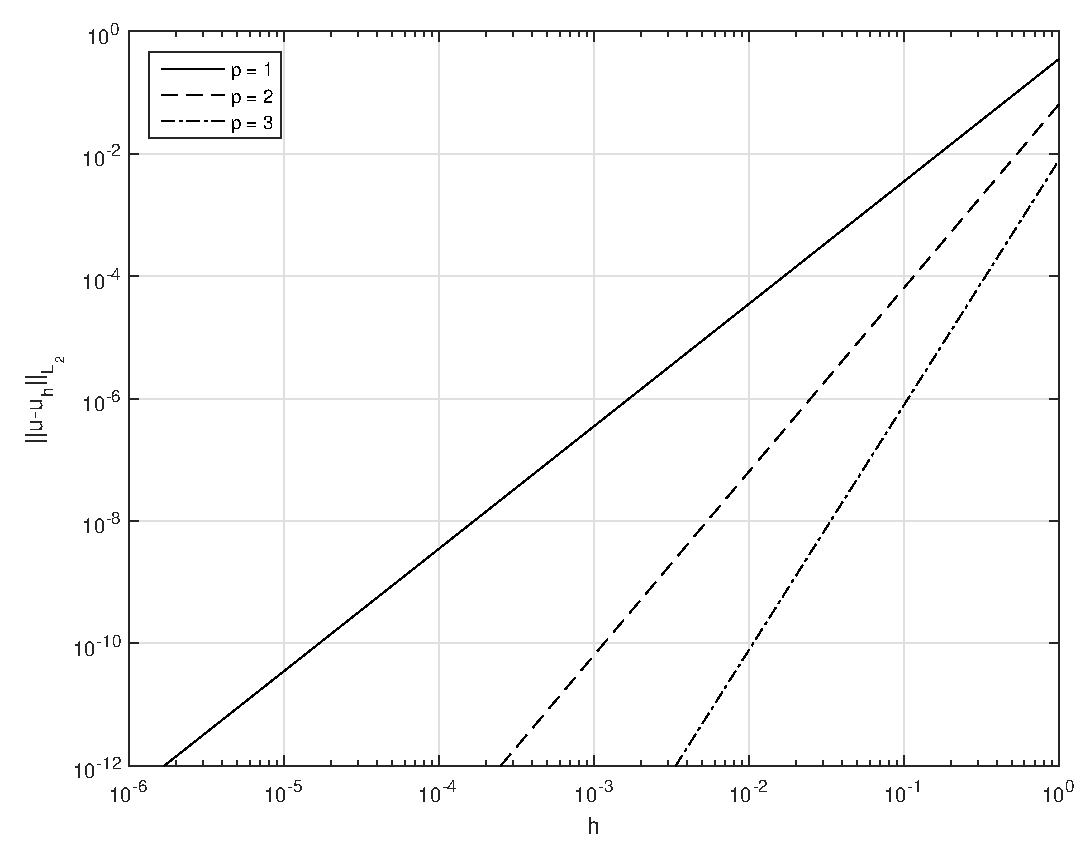
\includegraphics[width=\textwidth]{figures/sec_Sn/hConverge.eps}
	\end{subfigure}
	\begin{subfigure}[b]{0.495\textwidth}
		\centering
		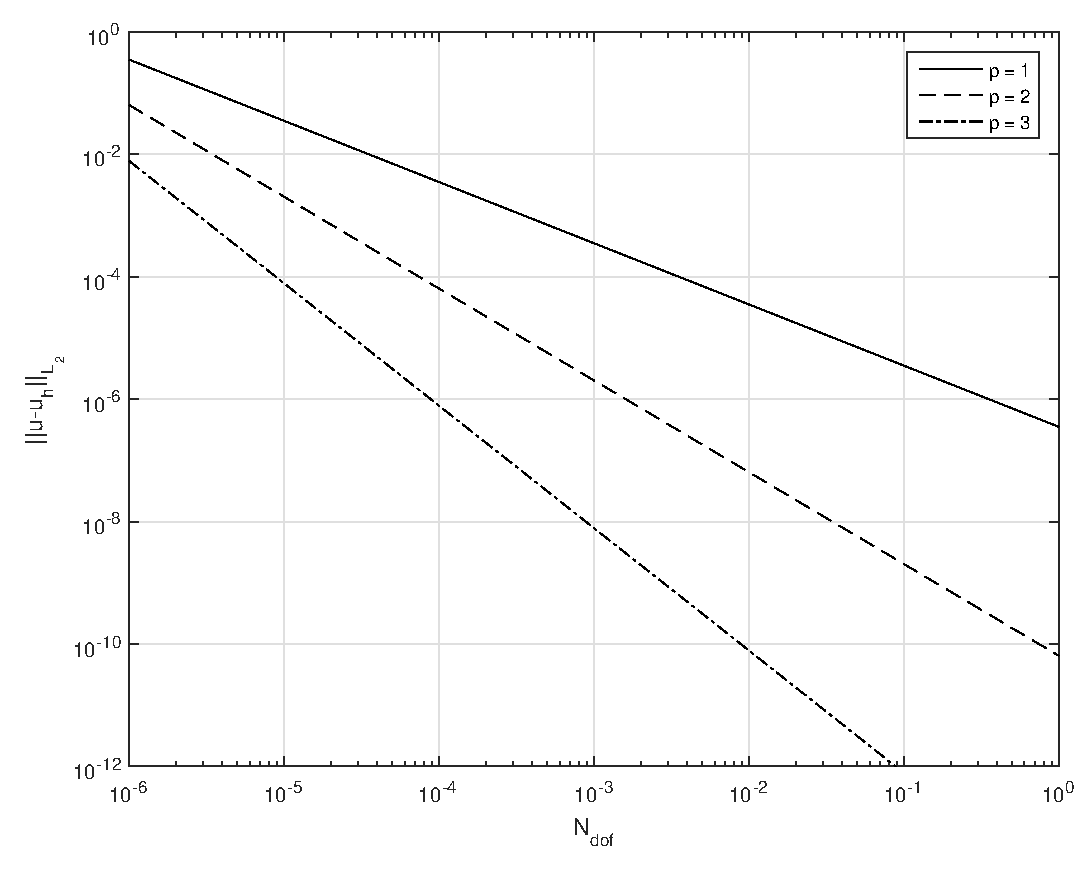
\includegraphics[width=\textwidth]{figures/sec_Sn/NConverge.eps}
	\end{subfigure}
\caption{Example of the theoretical convergence rates for a DGFEM transport problem that is not bound by solution regularity in terms of the maximum element diameter (left) and number of degrees of freedom (right).}
\label{fig::Sn_Spatial_Convergence}
\end{figure}
%%%%%%%%%%%%%%%%%%%%%%%%%%%%%%%%%%%%%%%%%%%%%%%%%%%
%%%   SubSection - Elementary
\subsection{Elementary Matrices on an Arbitrary Spatial Cell}
\label{sec::Sn_Spatial_Matrices}

In Eq. (\ref{eq::Sn_DGFEM_trans_eq_cellK_complete}), we presented the full set of spatially-discretized equations needed to solve the angular flux solution for cell $K$ for a single angular direction. In the equation, several terms of various types arise including interaction, $\Big( \sigma  b_m , \Psi_m  \Big)_K$, streaming, $ \Big( \vec{\Omega}_m \cdot \vec{\nabla}  b_m , \Psi_m  \Big)_K$, and surface, $     \Big< \left( \vec{\Omega}_m \cdot  \vec{n} \right) \, b_m, \Psi_m  \Big>_{\partial K}$. Each of these correspond to a different elementary matrix type. We now present how to compute the mass, streaming, and surface matrices in Sections \ref{sec::Sn_Spatial_Matrices_Mass}, \ref{sec::Sn_Spatial_Matrices_Streaming}, and \ref{sec::Sn_Spatial_Matrices_Surface}, respectively.

%%%%%%%%%%%%%%%%%%%%%%%%%%%%%%%%%%%%%%%%%%%%%%%%%%%
%%%   SubSection - Mass
\subsubsection{Elementary Mass Matrices}
\label{sec::Sn_Spatial_Matrices_Mass}

In the spatially discretized equations presented in Section \ref{sec::Sn_Spatial}, there are several reaction terms that appear with the form: $\Big( \sigma  b_m , \Psi_m  \Big)_K$ for a given angular direction, $m$, and for a spatial cell, $K$. In FEM analysis these reaction terms are ubiquitously referred to as the mass matrix terms \cite{zeinkiewicz2005finite,akin1982application}. For cell $K$, we define the elementary mass matrix, ${\bf M}$, as

\begin{equation}
\label{eq::Sn_mass_matrix_analytical}
{\bf M}_K =    \int_K {\bf b}_K \, {\bf b}_K^T \, d r ,
\end{equation}

\noindent where ${\bf b}_K$ corresponds to the set of $N_K$ basis functions that have non-zero measure in cell $K$. Depending on the FEM basis functions utilized, the integrals in Eq. (\ref{eq::Sn_mass_matrix_analytical}) can be directly integrated analytically. However, if in general, the basis functions cannot be analytically integrated on an arbitrary set of cell shapes, then a numerical integration scheme becomes necessary. If we define a quadrature set, $\left\{  \vec{x}_q , w_q^{K}  \right\}_{q=1}^{N_q}$, for cell $K$, consisting of $N_q$ points, $\vec{x}_q$, and weights, $w_q^K$, then we can numerically calculate the mass matrix by the following

\begin{equation}
\label{eq::Sn_mass_matrix_numerical}
{\bf M}_K = \sum_{q = 1}^{N_q} w_{q}^K {\bf b}_K (\vec{x}_q) \, {\bf b}_K^T (\vec{x}_q)  .
\end{equation}

\noindent In this case, it is necessary that the sum of the weights of this quadrature set exactly equal the geometric measure of cell $K$. This means that $\sum_{q = 1}^{N_q} w_{q}^K$ is equal to the cell width in 1 dimension, the cell area in 2 dimensions, and the cell volume in 3 dimensions.

Since ${\bf b}_K$ consists of a column vector for the basis functions and ${\bf b}_K^{T}$ consists of a row vector, then their multiplication will obviously yield a full $(N_K \, \text{x} \, N_K)$ matrix. This matrix is written for completeness of this discussion on the mass matrix:

\begin{equation}
\label{eq::Sn_mass_matrix_array}
{\bf M}_K =   \left[
\begin{array} {ccccc}
	\int_K b_1 \, b_1  & \ldots & \int_K b_1 \, b_j  & \ldots & \int_K b_1 \, b_{N_K} \\
	\vdots  &  & \vdots  &  & \vdots \\
	\int_K b_i \, b_1  & \ldots & \int_K b_i \, b_j  & \ldots & \int_K b_i \, b_{N_K} \\
	\vdots  &  & \vdots  &  & \vdots \\
	\int_K b_{N_K} \, b_1  & \ldots & \int_K b_{N_K} \, b_j  & \ldots & \int_K b_{N_K} \, b_{N_K} \\
\end{array}
\right] ,
\end{equation}

\noindent where an individual matrix entry is of the form:

\begin{equation}
\label{eq::Sn_mass_matrix_entry}
M_{i,j,K} =  \int_K b_i \, b_j .
\end{equation}

%%%%%%%%%%%%%%%%%%%%%%%%%%%%%%%%%%%%%%%%%%%%%%%%%%%
%%%   SubSection - Streaming
\subsubsection{Elementary Streaming Matrices}
\label{sec::Sn_Spatial_Matrices_Streaming}

Next, we will consider the streaming term that has the form: $ \Big( \vec{\Omega}_m \cdot \vec{\nabla}  b_m , \Psi_m  \Big)_K$ for a given angular direction, $m$, and for a spatial cell, $K$. $\vec{\nabla} $ is the gradient operator in physical space. It has the form of $\vec{\nabla} = \left[ \frac{d}{dx} \right]$ in 1 dimension, the form of $\vec{\nabla} = \left[ \frac{\partial}{\partial x} , \frac{\partial}{\partial y} \right]$ in 2 dimensions, and the form of $\vec{\nabla} = \left[ \frac{\partial}{\partial x} , \frac{\partial}{\partial y} , \frac{\partial}{\partial z} \right]$ in 3 dimensions. Since for every cell, the streaming term is applied for all $M$ angles in the angular discretization, we define the analytical elementary streaming matrix:

\begin{equation}
\label{eq::Sn_streaming_matrix_analytical}
\vec{{\bf G}}_K =    \int_K \vec{\nabla} {\bf b}_K \, {\bf b}_K^T \, d r ,
\end{equation}

\noindent which has dimensionality $(N_K \text{x} N_K \text{x} d)$. We choose to store the elementary streaming matrix in this form and not store $M$ separate $(N_K \text{x} N_K)$ local matrices corresponding to the application of the dot product ($ \vec{\Omega}_m  \cdot \int_K  \vec{\nabla} {\bf b}_K \, {\bf b}_K^T \, d r$). Instead, we simply evaluate the dot product with the appropriate angular direction whenever necessary. This has great benefit when trying to run large transport problems where memory becomes a premium and processor operations are not our limiting bottleneck. 

Just like the elementary mass matrix, we can use the same spatial quadrature set, $\left\{  \vec{x}_q , w_q^{K}  \right\}_{q=1}^{N_q}$, for cell $K$ to numerically calculate the streaming matrix:

\begin{equation}
\label{eq::Sn_streaming_matrix_numerical}
\vec{{\bf G}}_K =    \sum_{q = 1}^{N_q} w_{q}^K \vec{\nabla} {\bf b}_K (\vec{x}_q) \, {\bf b}_K^T (\vec{x}_q) .
\end{equation}

\noindent In this case, this local cell-wise streaming matrix has the full matrix form:

\begin{equation}
\label{eq::Sn_streaming_matrix_array}
\vec{{\bf G}}_K =   \left[
\begin{array} {ccccc}
	\int_K \vec{\nabla}b_1 \, b_1  & \ldots & \int_K \vec{\nabla}b_1 \, b_j  & \ldots & \int_K \vec{\nabla}b_1 \, b_{N_K} \\
	\vdots  &  & \vdots  &  & \vdots \\
	\int_K \vec{\nabla} b_i \, b_1  & \ldots & \int_K \vec{\nabla}b_i \, b_j  & \ldots & \int_K \vec{\nabla}b_i \, b_{N_K} \\
	\vdots  &  & \vdots  &  & \vdots \\
	\int_K \vec{\nabla} b_{N_K} \, b_1  & \ldots & \int_K \vec{\nabla} b_{N_K} \, b_j  & \ldots & \int_K \vec{\nabla} b_{N_K} \, b_{N_K} \\
\end{array}
\right] ,
\end{equation}

\noindent where an individual matrix entry is of the form:

\begin{equation}
\label{eq::Sn_streaming_matrix_entry}
\vec{G}_{i,j,K} =  \int_K \vec{\nabla}b_i \, b_j .
\end{equation}

%%%%%%%%%%%%%%%%%%%%%%%%%%%%%%%%%%%%%%%%%%%%%%%%%%%
%%%   SubSection - Surface
\subsubsection{Elementary Surface Matrices}
\label{sec::Sn_Spatial_Matrices_Surface}

Finally, the last terms to consider of the discretized transport equation are those found on the faces of the cell boundary: $  \vec{\Omega}_m \cdot  \Big<  \vec{n} \, b_m, \Psi_m  \Big>_{\partial K}$. These terms are analogous to the cell mass matrix but are computed on the cell boundary with dimensionality $(d-1)$. Analyzing a single face, $f$, in cell $K$, the analytical surface matrix is of the form,

\begin{equation}
\label{eq::Sn_surface_matrix_analytical}
\vec{{\bf F}}_{f,K}  =    \int_f \vec{n} (\vec{r}) \, {\bf b}_K \, {\bf b}_K^T \, d s ,
\end{equation}

\noindent where we allow the outward surface normal, $\vec{n}$, to vary along the cell face. For 1D problems as well as 2D problems with colinear cell faces (no curvature), the outward normals would be constant along the entire face. However, there are many cases where 3D mesh cells would not have coplanar vertices along a face. Then, the outward normal would not be constant along the face and would need to be taken into account during integration procedures. A simple example of non-coplanar face vertices would be an orthogonal hexahedral cell that has its vertices undergo a randomized displacement.

With the analytical form of the surface matrices defined in Eq. (\ref{eq::Sn_surface_matrix_analytical}), we can see that they have dimensionality, $(N_K \text{x} N_K \text{x} d)$. This is the same dimensionality as the cell streaming term. However, it is possible to reduce the dimensionality of the surface matrices if it is desired to reduce the memory footprint. There are some basis sets where all but $N_b^{f,K}$ basis functions are zero along face $f$. If we also restrict the mesh cell faces of our transport problems to have colinear (in 2D) or coplanar (in 3D) vertices so that the outward normal is constant along a face $f$, then we can define the surface matrix as $\int_f {\bf b}_K \, {\bf b}_K^T \, d s$. For these basis sets with $N_b^{f,K}$ non-zero face values on colinear/coplanar face $f$, the surface matrix has reduced dimensionality of $(N_b^{f,K} \text{x} N_b^{f,K})$.

Just like the cell mass and streaming matrices, it is possible that the basis functions cannot be integrated analytically. Analogous to the cell-wise quadrature, we can define a quadrature set for face $f$: $\left\{  \vec{x}_q , w_q^{f}  \right\}_{q=1}^{N_q^f}$. This quadrature set is not specific for just one of the cells that face $f$ separates. If the quadrature set can exactly integrate the basis functions of both cells $K$ and $K'$ (as defined by Figure \ref{fig::Sn_two_ref_cells}), then only 1 quadrature set needs to be defined for both cells. Using this quadrature set, we can numerically calculate the surface matrix for face $f$ along cell $K$:

\begin{equation}
\label{eq::Sn_surface_matrix_numerical}
\vec{{\bf F}}_{f,K} =    \sum_{q = 1}^{N_q^f} w_{q}^f \vec{n} (\vec{x}_q) \, {\bf b}_K (\vec{x}_q) \, {\bf b}_K^T (\vec{x}_q) .
\end{equation}

\noindent Similar to the cell-wise spatial quadrature sets, the sum of the weights of these face-wise quadrature sets needs to exactly equal the geometric measure of face $f$. This means that $\sum_{q = 1}^{N_q^f} w_{q}^f$ is equal to 1.0 in 1 dimension, the length of the face edge in 2 dimensions and the face area in 3 dimensions. 

Using the same notation as the cell-wise mass and streaming matrices, the local face-wise surface matrix for face $f$ has the full matrix form,

\begin{equation}
\label{eq::Sn_surface_matrix_array}
\vec{{\bf F}}_{f,K} =   \left[
\begin{array} {ccccc}
	\int_f \vec{n} \, b_1 \, b_1  & \ldots & \int_f \vec{n} \, b_1 \, b_j  & \ldots & \int_f \vec{n} \, b_1 \, b_{N_K} \\
	\vdots  &  & \vdots  &  & \vdots \\
	\int_f \vec{n} \,  b_i \, b_1  & \ldots & \int_f \vec{n} \, b_i \, b_j  & \ldots & \int_f \vec{n} \, b_i \, b_{N_K} \\
	\vdots  &  & \vdots  &  & \vdots \\
	\int_f \vec{n} \,  b_{N_K} \, b_1  & \ldots & \int_f \vec{n} \,  b_{N_K} \, b_j  & \ldots & \int_f \vec{n} \,  b_{N_K} \, b_{N_K} \\
\end{array}
\right] ,
\end{equation}

\noindent where an individual matrix entry is of the form:

\begin{equation}
\label{eq::Sn_surface_matrix_entry}
\vec{{ F}}_{i,j,f,K} =  \int_f \vec{n} \, b_i \, b_j .
\end{equation}

%%%%%%%%%%%%%%%%%%%%%%%%%%%%%%%%%%%%%%%%%%%%%%%%%%%
%%%   Section - Solution Procedures
\section{Solution Procedures}
\label{sec::Sn_Solution}

To this point, we have properly described the procedures to discretize the transport problem in energy, angle, and space. Combining the results of Sections \ref{sec::Sn_MG}, \ref{sec::Sn_Angle}, and \ref{sec::Sn_Spatial}, we write the fully-discretized DGFEM multigroup $S_N$ equations for an element $K$, where the test function $b_{m,g}$ for a single direction and energy group is now used:

\begin{equation}
\label{eq::Sn_DGFEM_trans_eq_cellK_bmg_complete}
\begin{aligned}
-  \Big( \vec{\Omega}_m \cdot  & \vec{\nabla} b_{m,g}, \Psi_{m,g} \Big)_{K}   + \Big(  \sigma_{t,g} b_{m,g} ,   \Psi_{m,g} \Big)_{K} +  \Big< ( \vec{\Omega}_m \cdot \vec{n} ) \, b_{m,g}, {\Psi}_{m,g}^{-}  \Big>_{\partial K^+}  \\
  + & \Big< ( \vec{\Omega}_m \cdot \vec{n} ) \, b_{m,g}, {\Psi}_{m,g}^{+}  \Big>_{\partial K^- \backslash \partial \mathcal{D}}  + \Big< ( \vec{\Omega}_m \cdot \vec{n} ) \, b_{m,g}, {\Psi}^{-}_{m',g}  \Big>_{\partial K^- \cap \partial \mathcal{D}^r}  \\
= & \sum\displaylimits_{g'=1}^G \sum_{p=0}^{N_P} \frac{2p + 1}{4 \pi} \sum_{n=-p}^{p}   Y_{p,n} (  \vec{\Omega}_m )  \Big( \sigma_{s,p}^{g' \rightarrow g} \, b_{m,g},  \Phi_{p,n,g'} \Big)_{K}  \\
+ & \left(  b_{m,g} ,   Q_{m,g} \right)_{K} - \Big< ( \vec{\Omega}_m \cdot \vec{n} ) \, b_{m,g}, {\Psi}_{m,g}^{inc}  \Big>_{\partial K^- \cap \partial \mathcal{D}^d}
\end{aligned} .
\end{equation} 

\noindent All of the notations used in Eq. (\ref{eq::Sn_DGFEM_trans_eq_cellK_bmg_complete}) remain unchanged from Section \ref{sec::Sn_Spatial}.

We now spend the remainder of this chapter discussing various methodologies to efficiently solve the tightly-coupled system of equations composing our transport problem. Section \ref{sec::Sn_Solution_Iterative} details the iterative procedures used to solve the transport problem in energy and angle, and Section \ref{sec::Sn_Solution_Spatial} then describes how we solve the spatial portion of the problem for a single energy/angle iteration.

%%%%%%%%%%%%%%%%%%%%%%%%%%%%%%%%%%%%%%%%%%%%%%%%%%%
%%%   SubSection - Iterative Procedures
\subsection{Angle and Energy Iteration Procedures}
\label{sec::Sn_Solution_Iterative}

The fully discretized transport equation has an angular flux solution, ${\bf \Psi}$, with dimensionality of $(G \text{x} M \text{x} N_{dof})$. The angular flux moments, ${\bf \Phi}$, have dimensionality of $(G \text{x} N_{mom} \text{x} N_{dof})$. Depending on the necessary fidelity of the problem, the full phase-space of the solution can become extremely large to solve. We can have {\em billions} of total unknowns to solve for if we simply have $N_{dof} \approx O(10^6)$, $M \approx O(10^2)$, and $G \approx O(10^1)$. These orders of number of unknowns in space, angle, and energy are of reasonable size for 3D transport problems.

In theory, if we had the computer memory, we could construct a left-hand-side matrix of dimensionality $(G \text{x} M \text{x} N_{dof})$x$(G \text{x} M \text{x} N_{dof})$ with a corresponding right-hand-side vector of dimensionality $(G \text{x} M \text{x} N_{dof})$x1, and we could then directly solve for the full phase-space angular flux solution at once. However, because the dimensional space of the unknowns can rapidly grow and become too large for hardware memory, transport problems have traditionally been solved iteratively. We now detail the procedures that we will employ to iteratively obtain the phase-space solution in energy and angle.

Because of the tight coupling that arises between the set of multigroup $S_N$ equations is between the energy groups in the scattering source, our iterative procedures principally lie in the energy domain. Figure \ref{fig::Sn_Solution_Iterative_scattmatrix} presents a pair of scattering matrices that show typical coupling between energy groups for neutronics problems. Depending on how the group boundaries are established along with a possible need for higher fidelity in energy, thermal upscattering may or may or may not be present in the problem. We can see from Figure \ref{fig::Sn_Solution_Iterative_scattmatrix} that the purely-downscattering matrix only has 1-way coupling, from high-to-low in the group energies. This means that if we progress through the energy groups from $g=1,...,G$ (in what is called an {\em outer iteration}), then we only have to do so once and we are done. However, there are many transport problems where we wish to have several energy groups in the thermal region. This leads to thermal neutron upscattering and causes the lower-right portion of the scattering matrix to be full as seen in the bottom of Figure \ref{fig::Sn_Solution_Iterative_scattmatrix}. Then, depending on how the groups are structured, multiple outer iterations may be necessary to fully converge the scattering source.


\begin{figure}
\centering
	\begin{subfigure}[b]{0.58\textwidth}
		\centering
		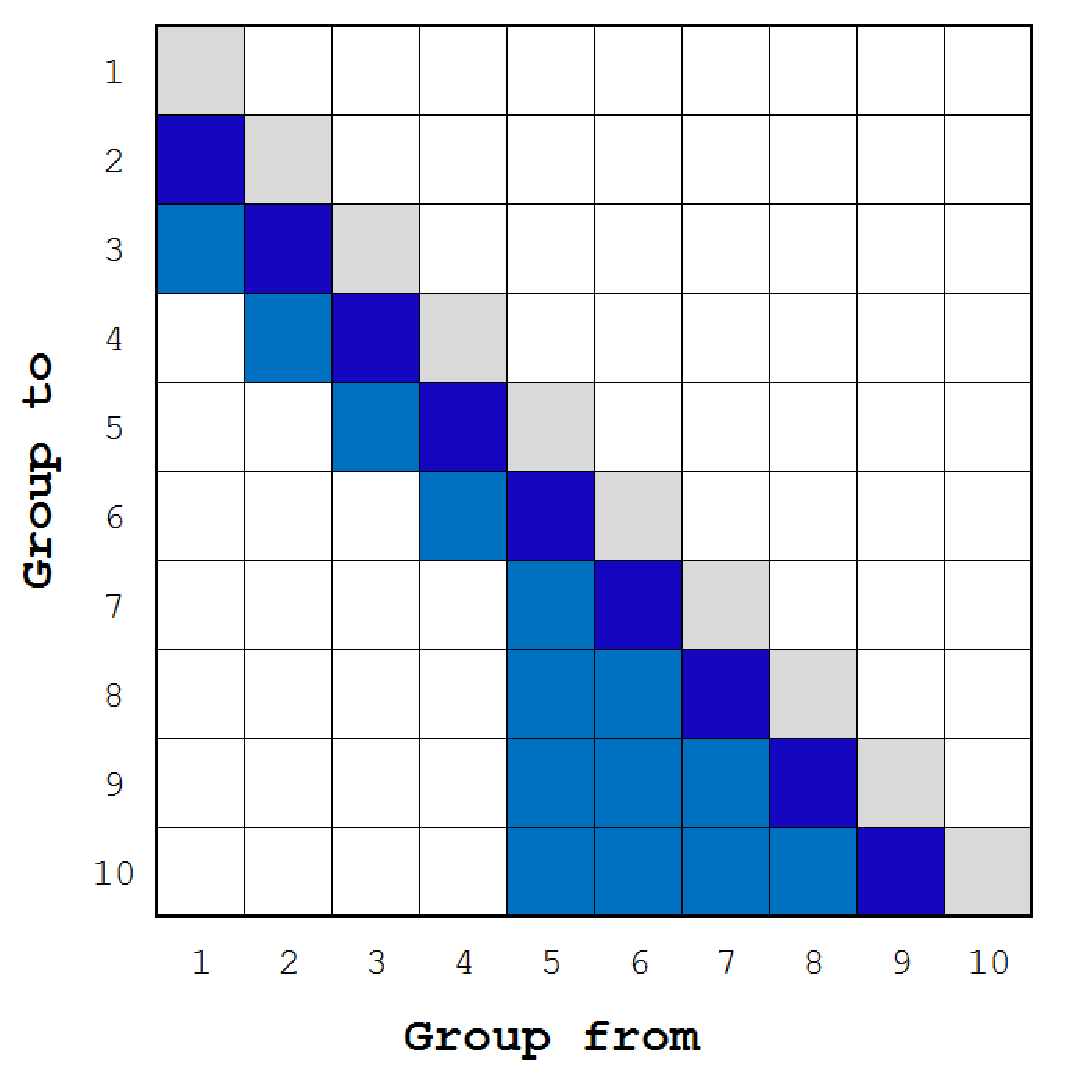
\includegraphics[width=\textwidth]{figures/sec_Sn/scattering_matrix_NO_upscattering.eps}
		\vspace{4mm}
	\end{subfigure}
	\hfill
	\begin{subfigure}[b]{0.58\textwidth}
		\centering
		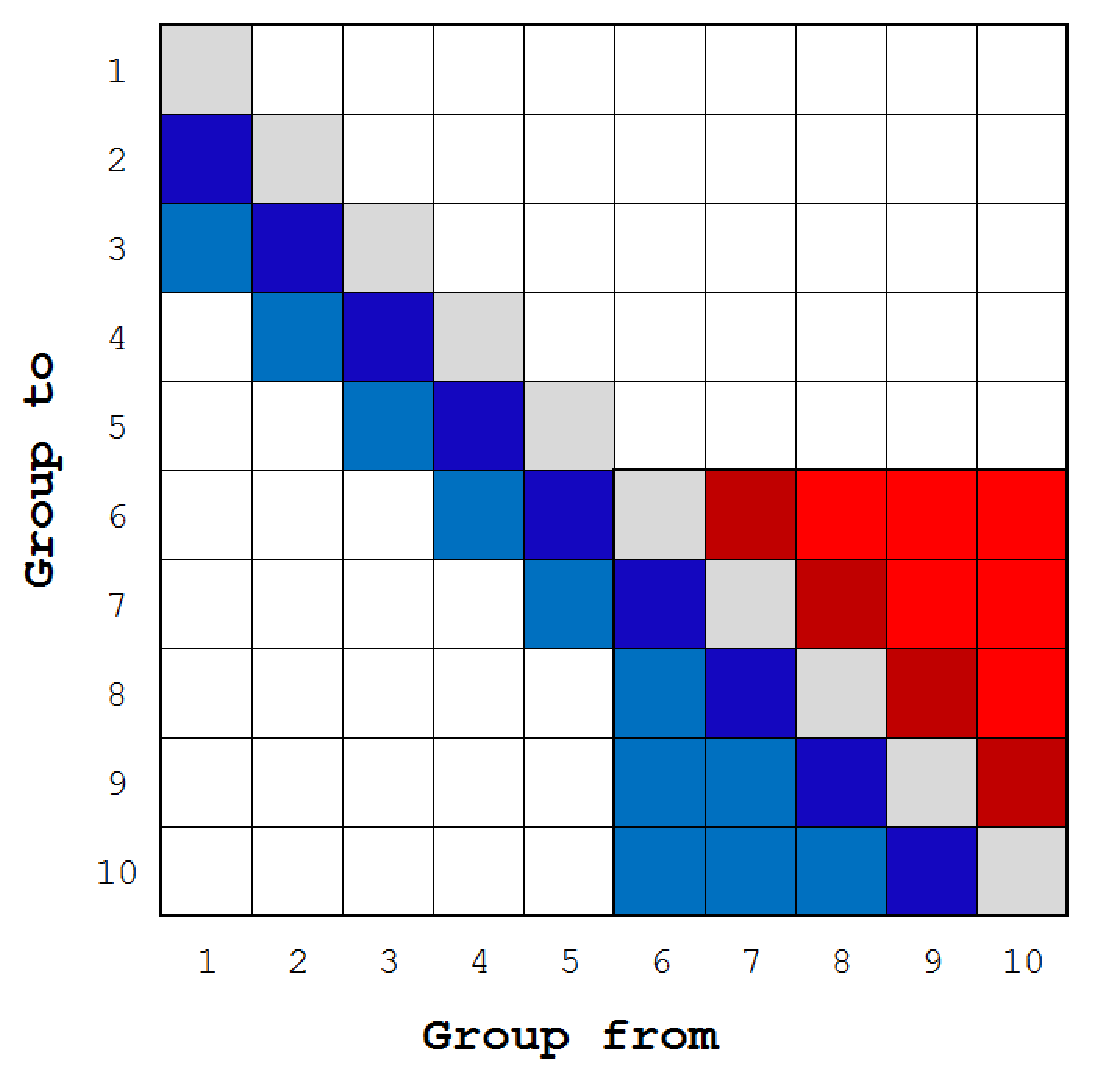
\includegraphics[width=\textwidth]{figures/sec_Sn/scattering_matrix_w_upscattering.eps}
	\end{subfigure}
\caption{Scattering matrices (top) without and (bottom) with upscattering. The gray corresponds to within-group scattering; the blue corresponds to down-scattering in energy; and the red corresponds to up-scattering in energy.}
\label{fig::Sn_Solution_Iterative_scattmatrix}
\end{figure}

We now describe the full iterative procedures required to converge the scattering source in detail. We begin by defining a new concept called a {\em group set}, which is simply a collection of contiguous groups. The group sets are ordered from high-to-low energy just like the groups and are non-overlapping with the adjoining sets. We demonstrate this concept with a simple example. If we have a problem with 10 groups ($G=10$), we then choose to aggregate them into 3 group sets. Group set 1 contains $g \in [1,3]$, group set 2 contains $g \in [4,7]$, and group set 3 contains $g \in [8,10]$. With these group sets defined, we then choose to employ a double iteration loop to converge the scattering source. The outer iterations in this procedure perform residual calculations by looping through the group sets. Then, for each group set in every outer iteration, {\em inner iterations} are performed. These inner iterations perform residual calculations to solve the scattering source within that group set to some specified tolerance. We will sometimes refer to these inner iterations as {\em within-group-set} (WGS) {\em iterations}. Because each outer iteration performs residual calculations for every group set, we will sometimes refer to these outer iterations as {\em across-group-set} (AGS) {\em iterations}. We continue performing AGS iterations until the solution residual is below some specified tolerance. At each outer and inner iteration, we possibly perform some acceleration (or preconditioning) step, where we leave the details for this until Chapter \ref{sec::DSA}. This complete iterative procedure involving the outer and inner iteration loops is given in Algorithm \ref{alg::Sn_Linear_Transport_Solve}. In this algorithm, we solve $N_{gs}$ number of group sets by using a maximum number of AGS iterations, $I_{ags}$, as well as a maximum number of WGS iterations for each group set, $I_{wgs}$.

As previously stated, the residual iterations for each group set only converge the scattering source for that group set. This means that the scattering sources from the other group sets are not modified during these iterations. We show this behavior by decomposing the transport equation into $N_{gs}$ separate equations where we have decomposed the scattering source into group set and across-group set components. The equations for the angular flux and flux moment solutions for each group set are given by

\begin{equation}
\label{eq::Sn_full_sol_gs_ops_psi}
\begin{aligned}
{\bf L}_{gs} {\bf \Psi}_{gs} =    {\bf M}_{gs} {\bf \Sigma}_{gs} {\bf \Phi}_{gs} + {\bf M}_{gs} \sum\displaylimits_{ggs \neq gs}  {\bf \Sigma}_{ggs} {\bf \Phi}_{ggs}+ {\bf Q}_{gs}  \\
gs=1,...,N_{gs}
\end{aligned} ,
\end{equation}

\noindent and

\begin{equation}
\label{eq::Sn_full_sol_gs_ops_phi}
{\bf \Phi}_{gs} =  {\bf D}_{gs} {\bf \Psi}_{gs} ,
\end{equation}

\noindent respectively, where ${\bf L}$ is the fully-discretized loss operator which consists of total interaction and streaming terms, ${\bf M}$ is the moment-to-discrete operator of the angular discretization, ${\bf D}$ is the discrete-to-moment operator of the angular discretization, ${\bf \Sigma}$ is the scattering operator of the multigroup and angular discretizations, and ${\bf Q}$ is the full phase-space distributed source. In this case, the source contains contributions from boundary, domain sources, and fission sources. We note that ${\bf M}$ and ${\bf D}$ are also group set dependent since we do not enforce the exact same angular discretization on all group sets. This can be useful if certain ranges of energy groups require higher angular fidelity due to increased anisotropic scattering.

We can further express Eq. (\ref{eq::Sn_full_sol_gs_ops_psi}) in terms of only the flux moments. Through algebra and linear algebra techniques, we state the flux-moment-only equation as

\begin{equation}
\label{eq::Sn_full_sol_moments_only}
\left( {\bf I} -{\bf T}_{gs} \right) {\bf \Phi}_{gs} = {\bf D}_{gs} {\bf L}_{gs}^{-1}  {\bf M}_{gs} \sum\displaylimits_{ggs \neq gs}  {\bf \Sigma}_{ggs} {\bf \Phi}_{ggs} +  {\bf D}_{gs} {\bf L}_{gs}^{-1}  {\bf Q}_{gs} ,
\end{equation}

\noindent where we define,

\begin{equation}
\label{eq::Sn_trans_op_T}
{\bf T}_{gs} \equiv {\bf D}_{gs} {\bf L}_{gs}^{-1}{\bf M}_{gs} {\bf \Sigma}_{gs} ,
\end{equation}

\noindent for further brevity. In Eqs. (\ref{eq::Sn_full_sol_moments_only}) and (\ref{eq::Sn_trans_op_T}), the term ${\bf L}_{gs}^{-1}$ accounts for the inversion of the loss operator. For this work, we will utilize the full-domain transport sweep, and we leave its details until Section \ref{sec::Sn_Solution_Spatial}. We now provide the details for the procedures that will be used to solve Eq. (\ref{eq::Sn_full_sol_moments_only}) in Sections \ref{sec::Sn_Solution_Iterative_SI} and \ref{sec::Sn_Solution_Iterative_GMRES}.

\begin{algorithm}
\caption{Iterative Solver in Energy for the Multigroup Transport Problem}
\label{alg::Sn_Linear_Transport_Solve}
\begin{algorithmic}[1]
\State Initialize: $\Phi_{g,p,n} = 0, \qquad g=1,...,G; \, p=0,...,N_p; \, n=-p,...,p$
\For{$a=1,...,I_{ags}$}
	\State {\bf Loop}: through group sets
	\For{$gs=1,...,N_{gs}$}
		\For{$k=1,...,I_{wgs}$}
			\State {\bf Perform}: residual iteration
			\State {\bf Apply}: Acceleration for group set $gs$
			\State {\bf Check}: convergence of group set $gs$
		\EndFor
	\EndFor
	\State {\bf Perform}: residual iteration
	\State {\bf Apply}:  Acceleration for across-group-set
	\State {\bf Check}: across-group-set convergence
\EndFor
\end{algorithmic}
\end{algorithm}

%%%%%%%%%%%%%%%%%%%%%%%%%%%%%%%%%%%%%%%%%%%%%%%%%%%
%%%   SubSubSection - Source Iteration
\subsubsection{Source Iteration}
\label{sec::Sn_Solution_Iterative_SI}

One simple method to invert the $({\bf I} - {\bf T})$ operator of Eq. (\ref{eq::Sn_full_sol_moments_only}) is the {\em source iteration} technique (SI), also known as {\em Richardson iteration}. If we isolate a single group set, $gs$, then the iterative procedure for the transport equation is

\begin{equation}
\label{eq::Sn_pre_si_iter}
{\bf L} {\bf \Psi}^{(k+1)} =    {\bf M} {\bf \Sigma} {\bf \Phi}^{(k)} +  {\bf Q} ,
\end{equation}

\noindent where we removed the $gs$ subscripts for brevity and note that the driving source ${\bf Q}$ contains scattering sources from all other group sets into the current group set of interest. From Eq. (\ref{eq::Sn_pre_si_iter}), we can see that the scattering source at iteration $(k+1)$ is calculated from a previous guess for the flux moments at iteration $(k)$. This is exactly a Jacobi iteration in energy for the group set. Then, after the application of one transport sweep, we obtain a new guess for the angular flux moments:

\begin{equation}
\label{eq::Sn_si_iter}
\begin{aligned}
 {\bf \Psi}^{(k+1)} &= {\bf L}^{-1} \left(  {\bf M} {\bf \Sigma} {\bf \Phi}^{(k)} +  {\bf Q} \right) \\
{\bf \Phi}^{(k+1)} &=  {\bf D} {\bf \Psi}^{(k+1)}
\end{aligned} .
\end{equation}

We continue to perform these Richardson iterations until the difference between two iterate solutions is less than some specified tolerance in a given norm. This convergence criterion for SI can be succinctly written as

\begin{equation}
\label{eq::Sn_SI_conv_crit}
\frac{|| \Phi^{(k+1)} - \Phi^{(k)} ||}{|| \Phi^{(k+1)} ||} \leq \text{tol} ,
\end{equation}

\noindent where the estimate for the error is normalized by the norm of the most recent iteration solution. Steps are taken to ensure that a divide-by-zero does not occur. In general, SI is guaranteed to converge for a large range of transport problems (further precautions need to be taken for problems with high anisotropic scattering). We can estimate how quickly SI will converge by analyzing the spectral radius (SR) of the transport problem \cite{ref::adams_larsen_iter_methods}. This spectral radius, $\rho$, can be estimated in the asymptotic convergence region by the ratio of two successive solution differences:

\begin{equation}
\label{eq::Sn_SI_SR_est}
\rho \approx \frac{|| \Phi^{(k+1)} - \Phi^{(k)} ||}{|| \Phi^{(k)} - \Phi^{(k-1)} ||} 
\end{equation}

\noindent We can gather a lot of information about how our transport solution will converge from Eq. (\ref{eq::Sn_SI_SR_est}). If $\rho>1$ in the asymptotic region, then the error in our residual will grow without end, and our solution will diverge. However, in the preasymptotic region, Eq. (\ref{eq::Sn_SI_SR_est}) may be a bad estimate for the spectral radius, and values greater than 1 may be observed for several iterations. This does not mean that the solution will diverge in the end. If we are in the asymptotic region, then we would like $\rho \ll 1$ because it means that our transport solution will quickly converge. However, if $\rho \approx 1$ (but still strictly less than 1), then our transport problem will slowly converge to our final solution. We demonstrate this behavior in Table \ref{tab::Sn_convergece_rates} by giving the average number of SI iterations required to reduce our solution error by 1 order of magnitude. We can see that as $\rho$ approaches 1, the iteration numbers become prohibitively large. For those problems with large spectral radii, we can accelerate our solution convergence by using synthetic acceleration on Preconditioned Richardson Iteration \cite{ref::adams_larsen_iter_methods}. We leave the details for this in Chapter \ref{sec::DSA}.

\begin{table}
\caption{Average number of iterations required to reduce SI error by 1 order of magnitude for different SR values.}
\centering
%\begin{center}
\begin{tabular}{|c|c|}
\hline
$\rho$ & Iterations \\ \hline \hline
0.1 & 1.0 \\ 
0.25 & 1.6 \\ 
0.5 & 3.3 \\  
0.75 & 8.0 \\ 
0.9 & 22 \\ 
0.99 & 230 \\ 
0.999 & 2301 \\ 
0.9999 & 23024 \\
\hline
\end{tabular}
%\end{center}
\label{tab::Sn_convergece_rates}
\end{table}

%%%%%%%%%%%%%%%%%%%%%%%%%%%%%%%%%%%%%%%%%%%%%%%%%%%
%%%   SubSubSection - Krylov
\subsubsection{Krylov Subspace Methods}
\label{sec::Sn_Solution_Iterative_GMRES}

Source iteration is not the only iterative technique that can be employed to invert $({\bf I} - {\bf T})$ for a given group set. In the last 20 years, Krylov subspace methods have been applied to the discretized transport equation \cite{oliveira1998preconditioned,guthrie1999gmres,patton2002application}. Because $({\bf I} - {\bf T})$ is not symmetric, we want to only use Krylov methods that can solve non-symmetric matrices. The two Krylov subspace methods that we would naturally want to employ are GMRES and BiCGSTAB \cite{saad1986gmres,saad2003iterative}. We will not describe the implementations of these methods here for brevity. However, we will state that most of the computational machinery required to perform Richardson iterations can also be used for these Krylov methods. The only modifications/extensions that are needed are summarized in the following list.

\begin{enumerate}
\item Construction of the right-hand-side: ${\bf b} = {\bf D} {\bf L}^{-1} {\bf Q}$. From this equation, it is obvious that we need just one initial transport sweep to properly build this right-hand-side.
\item The operation of the matrix $({\bf I} - {\bf T})$ on a Krylov vector, $\nu$. This can easily be accomplished with the same machinery as Richardson iteration by simply subtracting the original flux moment vector by the updated moments after one transport sweep.
\item Modify the calculation of the convergence criterion so that the norm of the iteration residual, normalized by the right-hand-side, is smaller than some prescribed tolerance:
$\frac{||{\bf b} - ({\bf I} - {\bf T}) {\bf x} ||_2}{||{\bf b}||_2} < \text{tol}$.
\end{enumerate}

Combined with the appropriate linear algebra operations, these three small alterations are all that is required to properly utilize the Krylov solver for the transport equation. It is not immediately obvious how one would precondition the Krylov iterations in the context of transport sweeping. However, just like the Richardson iteration scheme, we will provide the implementation of DSA preconditioning for Krylov in Chapter \ref{sec::DSA}.

%%%%%%%%%%%%%%%%%%%%%%%%%%%%%%%%%%%%%%%%%%%%%%%%%%%
%%%   SubSection - Spatial Solution Procedures
\subsection{Spatial Solution Procedures}
\label{sec::Sn_Solution_Spatial}

Section \ref{sec::Sn_Solution_Iterative} presented the methodology that we will employ to iteratively converge our transport solutions in energy and angle (flux moments). Both Richardson iteration and the Krylov methods were presented as methods that can invert the $({\bf I} - {\bf T})$ operator. In both of these iterative methods, the common operation of interest is the inversion of the loss operator (${\bf L}$). There are different techniques that could be used to perform this operation, including several matrix-dependent and matrix-free methodologies. For this work, the loss operator inversion on some unstructured mesh, $\mathbb{T}_h$, will be performed by use of the full-domain transport sweep as outlined next in Section \ref{sec::Sn_Solution_Spatial_Sweeping}. We then conclude our discussion on spatial solution procedures by briefly describing how we can utilize adaptive mesh refinement (AMR) to generate irregular polytope meshes (without hanging nodes in this work) in Section \ref{sec::Sn_Solution_Spatial_AMR}.

%%%%%%%%%%%%%%%%%%%%%%%%%%%%%%%%%%%%%%%%%%%%%%%%%%%
%%%   SubSubSection - Transport Sweeping
\subsubsection{Transport Sweeping}
\label{sec::Sn_Solution_Spatial_Sweeping}

Recall from earlier that the continuous definition of the loss operator for an angular direction $m$ and energy group $g$ is,

\begin{equation}
\label{sec::Sn_Solution_Spatial_loss_op}
L_{m,g} =  \vec{\Omega}_m \cdot   \vec{\nabla} + \sigma_{t,g} \,  ,
\end{equation}

\noindent where we suppress the spatial parameter for brevity. From the application of the test function, integration by parts of the streaming term, and the use of the upwind scheme as outlined in Section \ref{sec::Sn_Spatial}, we described the coupling between different mesh cells. The upwind scheme only couples the adjoining cells upwind of any given angular direction. This means that for a given mesh element, if the upwind cells have already had their angular fluxes updated for a given iteration, we then have all the information needed to solve for the new angular fluxes on the element. This means that if the task dependence graphs are well chosen for all directions, we can then invert the streaming operator by solving Eq. (\ref{eq::Sn_DGFEM_trans_eq_cellK_bmg_complete}) one cell at a time for a given group of angular directions. 

This cell-by-cell inversion of the streaming operator is known as a {\em transport sweep}. If we perform this inversion for all angular directions across the entire spatial domain without lagging, then it is called a full-domain transport sweep. The full-domain transport sweep is a beneficial matrix-free scheme because of the following:

\begin{itemize}
\item The iterative solver does not need to build any matrices explicitly but only requires the action of ${\bf L}^{-1}$.
\item Does not require the formation of $M$ separate matrices for each of the angular directions (for 1 energy group). This is both memory and computationally intensive for any problems of appreciable size.
\item The matrix-vector operations on a single element within a transport sweep can be efficiently performed depending on the group set structure and the angle aggregation as outlined in Section \ref{sec::Sn_Solution_Iterative}.
\item The matrix-free transport sweep favors higher-order DGFEM schemes since they will yield more processor work per element with less memory caching (which is the current bottleneck with massively-parallel calculations).
\item The number of sweep iterations does not grow with increasing problem size or processor counts. This is in contrast with partial-domain sweeping like {\em parallel block jacobi} (PBJ) \cite{zerr2011solution}.
\end{itemize}

\begin{figure}
\centering
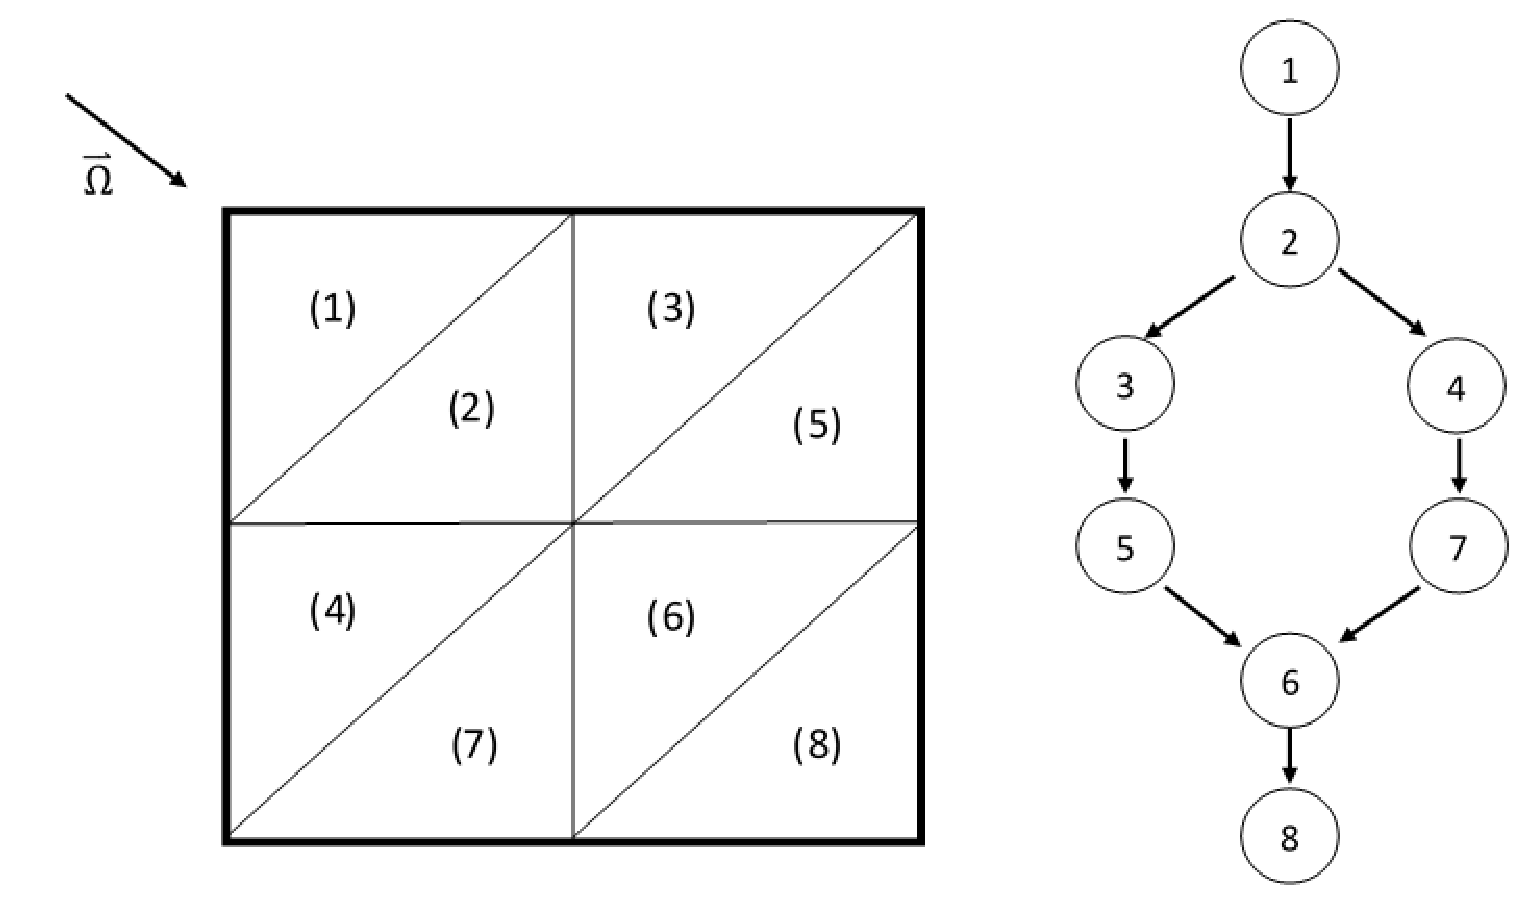
\includegraphics[width=0.70\textwidth]{figures/sec_Sn/triangle_graph_nocycle.eps}
\caption{Task dependence graph for the transport sweep for a given direction without cycles.}
\label{fig::Sn_Solution_Spatial_Sweeping_sweepNOcycle}
\end{figure}

\begin{figure}
\centering
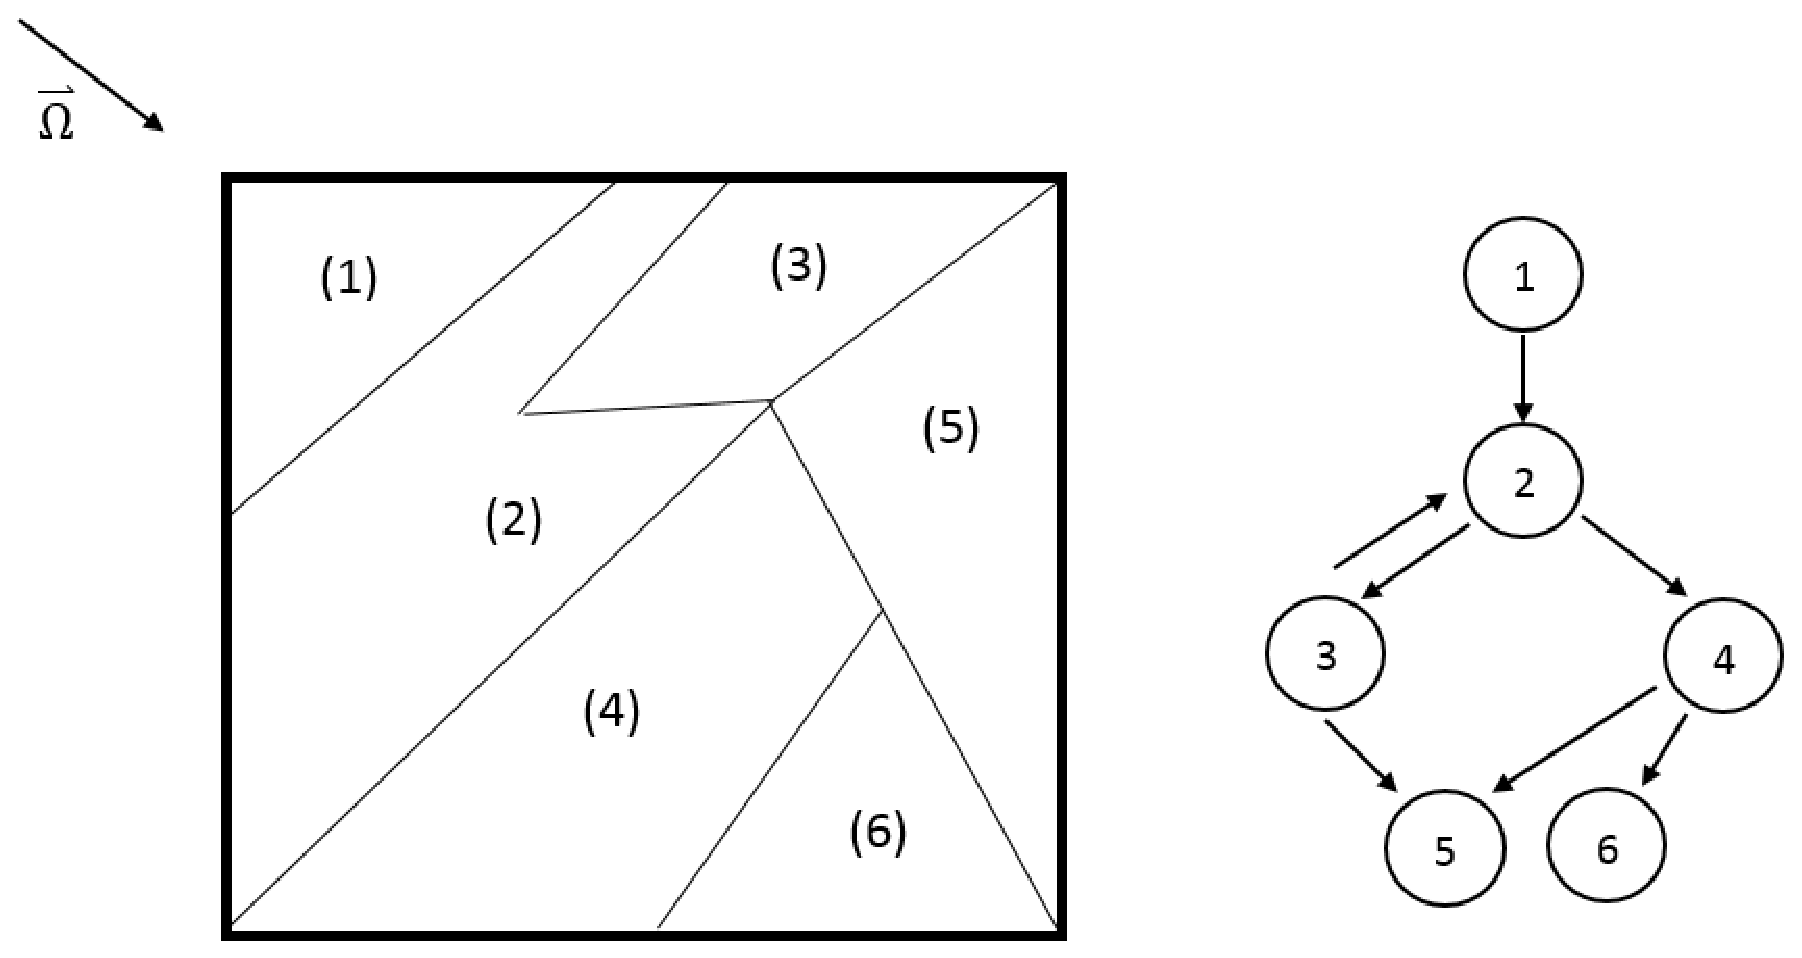
\includegraphics[width=0.70\textwidth]{figures/sec_Sn/graph_with_cycling.eps}
\caption{Task dependence graph for the transport sweep for a given direction with cycles present.}
\label{fig::Sn_Solution_Spatial_Sweeping_sweepWcycle}
\end{figure}

We can gain knowledge of how our transport sweeps will perform by analyzing the streaming operator, ${\bf L}$, in space and angle. If ${\bf L}$ is strictly block-lower triangular for a given angular direction, then it is guaranteed that an ordering of the mesh cells can be represented by a Directed Acyclic Graph (DAG) \cite{gerasoulis1989static}. However, situations can arise where a cycle forms in the graph and a complete sweep for those directions becomes impossible. These situations include concave polytope elements that cause re-entrance, opposing reflecting boundary conditions, and extreme distortion of an $\mathbb{R}^3$ domain (regular mesh of hexahedral cells with 1 dimensional end twisted). Figure \ref{fig::Sn_Solution_Spatial_Sweeping_sweepNOcycle} shows a DAG without any cycles for the given direction. Figure \ref{fig::Sn_Solution_Spatial_Sweeping_sweepWcycle} then shows a graph with a cycle caused by a re-entrant quadrilateral mesh cell. There are methods to break these cycles and still perform transport sweeping, but we will not consider them for this work.

Up to this point, we have provided the basic details on how a transport sweep is performed. We now switch our discussion to recent developments involving provably optimal sweeping algorithms with high efficiencies out to $O(10^5)$ - $O(10^6)$ processors. For over a decade, the Koch-Baker-Alcouffe (KBA) parallel sweeping algorithm was the most prevalent in the computational transport community \cite{ref::KBA,baker1998s}. The KBA algorithm spatially partitions the problem by assigning each processor a column of cells. During a transport sweep, the cell-by-cell solution of each angular direction is represented as a Task Dependence Graph (TDG). KBA operates by initializing a new TDG as soon as it completes a previous TDG for all directions in an octant-pair. This consecutive execution of TDGs is known as ``pipelining''. Unfortunately, KBA's pipelining penalty grows with processor counts but the TDG width grows only as $P^{2/3}$. Therefore, KBA eventually runs out of parallelism to exploit which led to the common belief that transport sweeps would not scale beyond $O(10^3)$ - $O(10^4)$ processing units.

Now we give an overview of a provably-optimal sweeping algorithm that will be utilized in this work \cite{ref::eff_sweeps,adams2013provably}. Consider a transport problem with a ($N_x \times N_y \times N_z $) spatial grid of Cartesian mesh cells and a ($P_x \times P_y \times P_z $) processor layout. Assume that $N_x/P_x$, $N_y/P_y$, and $N_z/P_z$ are all integer values. Now suppose a group set that we wish to sweep has $G$ groups and $M$ angular directions per octant. This means that each processor must perform $(8 M G N_x N_y N_z)/(P_x P_y P_z)$ total calculations for the transport sweep. We then aggregate these calculations into tasks with each task containing $A_g$ groups, $A_M$ directions and $A_x A_y A_z$ spatial cells. Therefore, each processor must perform $N_{tasks}$ number of tasks which can be given by

\begin{equation}
\label{sec::Sn_Solution_Spatial_Ntasks}
N_{tasks} = \frac{8 M G N_x N_y N_z}{A_g A_M A_x A_y A_z  P_x P_y P_z} .
\end{equation}

\noindent The complete transport sweep requires a total of $N_{stages}$ stages, given by

\begin{equation}
\label{sec::Sn_Solution_Spatial_Nstages}
N_{stages} = N_{tasks} + N_{idle} ,
\end{equation}

\noindent where $N_{idle}$ is the number of processor idle stages. Using these definitions, the parallel efficiency, $\epsilon$, of the sweep can be written as

\begin{equation}
\label{sec::Sn_Solution_Spatial_paralleleff}
\epsilon = \frac{1}{\left[ 1+\frac{N_{idle}}{N_{tasks}} \right] \, \left[ 1+\frac{T_{comm}}{T_{task}} \right]} ,
\end{equation}

\noindent where $T_{task}$ is the time required to complete a single task and $T_{comm}$ is the time required to communicate data after a task has completed. Minimizing the terms (as close to unity as possible) in the denominator will lead to higher parallel efficiencies. However, the bracketed terms compete against each other because maximizing $N_{tasks}$ will minimize $T_{task}$. 

For a given set partitioning parameters and aggregation factors, the minimum number of stages is $2 N_{fill} + N_{tasks}$, where $N_{fill}$ is the number of stages for a sweepfront to reach the center processors in the domain. If we set $A_x = N_x / P_x$ and $A_y = N_y / P_y$ and define $\delta_u =$ 0 or 1 for $P_u$ even or odd, respectively, and $N_k=N_z / (P_z A_z)$, then

\begin{equation}
\label{sec::Sn_Solution_Spatial_Nfill_Nidle}
\begin{aligned}
N_{fill} = \frac{P_x + \delta_x}{2} - 1 +  \frac{P_y + \delta_y}{2} - 1 + N_k \left( \frac{P_z \delta_z}{2} -1 \right) \\
N_{idle}^{min} = P_x + \delta_x - 2  P_y + \delta_y - 2 + N_k ( P_z + \delta_z - 2)
\end{aligned}
\end{equation}

\noindent and

\begin{equation}
\label{sec::Sn_Solution_Spatial_Nmin}
N_{stages}^{min} = N_{idle}^{min} + \frac{8 M G N_k}{A_M A_g}
\end{equation}

\noindent If the minimum stage count could be achieved, then the optimal parallel efficiency, $\epsilon_{opt}$, can be given by the following

\begin{equation}
\label{sec::Sn_Solution_Spatial_epopt}
\epsilon_{opt} = \frac{1}{\left[ 1+\frac{(P_x + \delta_x) + (P_x + \delta_x) - 4 + N_k ( P_z + \delta_z - 2)}{{8 M G N_k} / {(A_M A_g)}} \right] \, \left[ 1+\frac{T_{comm}}{T_{task}} \right]} .
\end{equation}



%%%%%%%%%%%%%%%%%%%%%%%%%%%%%%%%%%%%%%%%%%%%%%%%%%%
%%%   SubSubSection - AMR
\subsubsection{Spatial Adaptive Mesh Refinement}
\label{sec::Sn_Solution_Spatial_AMR}

Adaptive Mesh Refinement (AMR) techniques have become more commonplace across many scientific and engineering fields over the last couple of decades \cite{plewa2005adaptive,carey1997computational,ramm2003error,karniadakis2013spectral,schwab1998p,solin2003higher}. However, while this has become more common practice in other disciplines, the use of AMR for the transport equation is still in its infancy \cite{fuhrer1997posteriori,hartmann2002adaptive,dedner2002adaptive,hartmann2003adaptive,ragusa2010two,wang2011standard}. For this work, we will only utilize {\em h}-type refinement strategies for 2D transport problems on initial meshes with only quadrilateral cells. 

Figure \ref{fig::Sn_Solution_Spatial_AMR_flowchart} provides the logical flow chart used to perform the mesh adaptation procedures for our problem of interest. The AMR procedure begins with an initial and typically coarse mesh. The transport solution is calculated on this mesh with appropriate PDE solvers. Once this solution is determined, {\em a posteriori} error estimates are used to determine which problem regions contain the largest spatial discretization error \cite{verfurth1996review,ainsworth2011posteriori}. Then, based on some refinement criterion, some subset of mesh elements are flagged for local refinement. From these flagged elements, the mesh can be refined, and a new and more accurate solution can further be obtained. This process is repeated until some global convergence criterion is satisfied or some number of mesh adaptation cycles are performed.

\begin{figure}
\centering
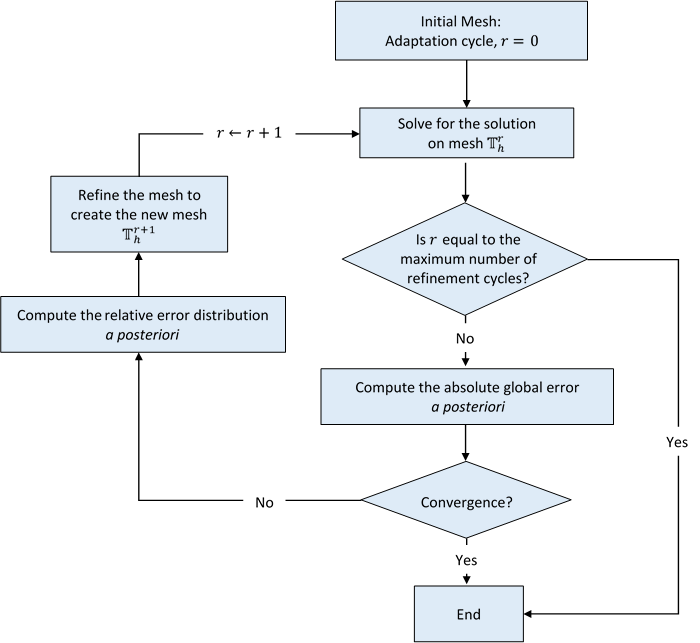
\includegraphics[width=0.95\textwidth]{figures/sec_Sn/AMR_Flow_Chart.png}
\caption{Flow chart for mesh adaptation.}
\label{fig::Sn_Solution_Spatial_AMR_flowchart}
\end{figure}

At the heart of the mesh adaptation procedures is the reliance on an accurate estimation of the numerical solution error. The state-of-the-art error estimators rely on either adjoint-based methods \cite{fuhrer1997posteriori,hartmann2002adaptive,hartmann2003adaptive} or projection-based methods \cite{demkowicz2006computing}. However, these methods require an additional calculation of the solution at each refinement level in a richer (and more difficult to solve) functional space. Therefore, we will employ a simpler error estimator that does not require an additional solution calculation. For this work, we will utilize the jump-based error estimator since it is the most straightforward to define and execute. The estimate of the error for mesh cell $K$ of the mesh at refinement level $r$, $\mathbb{T}_h^r$, is given by the following, 

\begin{equation}
\label{eq::Sn_AMR_jump_err_est}
\eta_K^r = \int\displaylimits_{\partial K} [\![ \Phi^r ]\!]^2 d \, s = \int\displaylimits_{\partial K} \left(  \sum_m w_m [\![ \Psi_m^r ]\!]  \right)^2 ,
\end{equation}

\noindent where $[\![ \cdot ]\!]$ is the jump operator along a face defined as,

\begin{equation}
\label{eq::Sn_AMR_jump_def}
[\![ \Phi (\vec{r}) ]\!] = \Phi^+ (\vec{r}) - \Phi^- (\vec{r}),
\end{equation}

\noindent and the terms, $\Phi^+ (\vec{r})$ and $\Phi^- (\vec{r})$, are subject to the trace:

\begin{equation}
\label{eq::Sn_AMR_jump_trace}
\Phi^{\pm} (\vec{r})  = \lim\displaylimits_{s \rightarrow 0^{\pm}} \Phi (\vec{r} + s \vec{n}).
\end{equation}

\noindent In this case, the outward normal, $\vec{n}$, is determined with respect to the element $K$ along its boundary, $\partial K$. With this trace, $\Phi^- (\vec{r})$ always corresponds to the solution within cell $K$. Investigating face $f$ of cell $K$, the across-face solution, $\Phi^+ (\vec{r})$, is dependent on the boundary type of face $f$. The across-face solutions can be succinctly written:

\begin{equation}
\label{eq::Sn_AMR_across_face_vals}
\Phi^+ (\vec{r}) = 
\begin{cases}
\lim\displaylimits_{s \rightarrow 0^{+}} \Phi (\vec{r} + s \vec{n}) & \vec{r} \notin \partial \mathcal{D} \\
\sum\displaylimits_{\vec{\Omega}_m \cdot \vec{n} > 0}  \Psi_m^- (\vec{r}) + \sum\displaylimits_{\vec{\Omega}_m \cdot \vec{n} < 0} \Psi_{m}^{inc} (\vec{r}) & \vec{r} \in \partial \mathcal{D}^d \\
\Phi^- (\vec{r}) & \vec{r} \in \partial \mathcal{D}^r
\end{cases}.
\end{equation}

\noindent From Eq. (\ref{eq::Sn_AMR_across_face_vals}), the across-face solutions for interior faces, incident boundaries and reflecting boundaries have different meanings. For an interior face $f$ ($\vec{r} \notin \partial \mathcal{D}$), the across-face solution comes from the cell $K'$ (as defined by Figure \ref{fig::Sn_two_ref_cells}). For incident boundaries ($\vec{r} \in \partial \mathcal{D}^d$), the across-face solution is a combination of integrals of the outgoing ($\Psi_m^-$) and incident boundary fluxes ($\Psi_m^{inc}$). Finally, for reflecting boundaries ($\vec{r} \in \partial \mathcal{D}^r$), the across-face solutions are simply the within-cell solutions. Therefore, the solution jump is exactly zero for all reflecting boundaries and yields no contribution to the error estimate.

With the error estimates defined for all cells $K \in \mathbb{T}_h^r$ for refinement level $r$, a criterion is needed to determine which cells should be refined. For this work, we choose to employ a refinement criterion of the following form,

\begin{equation}
\label{eq::Sn_AMR_err_crit}
\eta_K^r \geq \alpha \max\displaylimits_{K' \in \mathbb{T}_h^r} \left(  \eta_{K'}^{r} \right),
\end{equation}

\noindent where $\alpha$ is a user-defined value $(0,1)$. This refinement criterion has a simple meaning. If, for example, $\alpha = 0.2$, then a cell will be refined if its error estimate is greater than 20\% of the cell with the largest error estimate. This does not necessarily mean that 80\% of the mesh cells will be refined at level $r$. Instead, the criterion simply states that any cell above a particular threshold will be refined. This means that it is theoretically possible for the extreme cases of 1 or all cells being refined at a particular refinement cycle. The first extreme case could arise with a single spatial cell having a strong solution discontinuity stemming from a strong localized source. The second extreme case could arise when the intercell solution jumps are about equivalent stemming from an incredibly smooth discretized solution at that particular refinement cycle. We could also enforce a uniform refinement of all the spatial cells by setting $\alpha=0$.

Once we have determined which elements on mesh level $r$ to refine, we then form our new adapted mesh on level $r+1$ by a combination of logical refinement rules, hierarchical elements, and refinement trees. Each quadrilateral mesh cell with vertices flagged for refinement (which we denote as the parent element) is further subdivided into four smaller quadrilateral cells (which we denote as daughter elements I, II, III, and IV) that maintain the overall shape of the original mesh cell. If the parent element is denoted by the vertices (1), (2), (3), and (4), then the refinement rules, including the new local ordering of each daughter element's vertices, are given in Figure \ref{fig::Sn_Solution_Spatial_AMR_quadrefrules}. These refinement rules are detailed as follows:

\begin{enumerate}
\item Daughter element I is placed near original vertex (1).
\item Daughter element II is placed near original vertex (2).
\item Daughter element III is placed near original vertex (3).
\item Daughter element IV is placed near original vertex (4).
\item The local numbering of the daughter element vertices is consistent with the parent element.
\item The vertices of the daughter elements common with the original element inherit the same local numbering.
\end{enumerate}

\noindent These refinement rules guarantee that we will maintain logical consistency with our counter-clockwise ordering of the element vertices. This consistency is important for the computation of the polytope basis functions that are presented in Chapter \ref{sec::BF}.

\begin{figure}
\centering
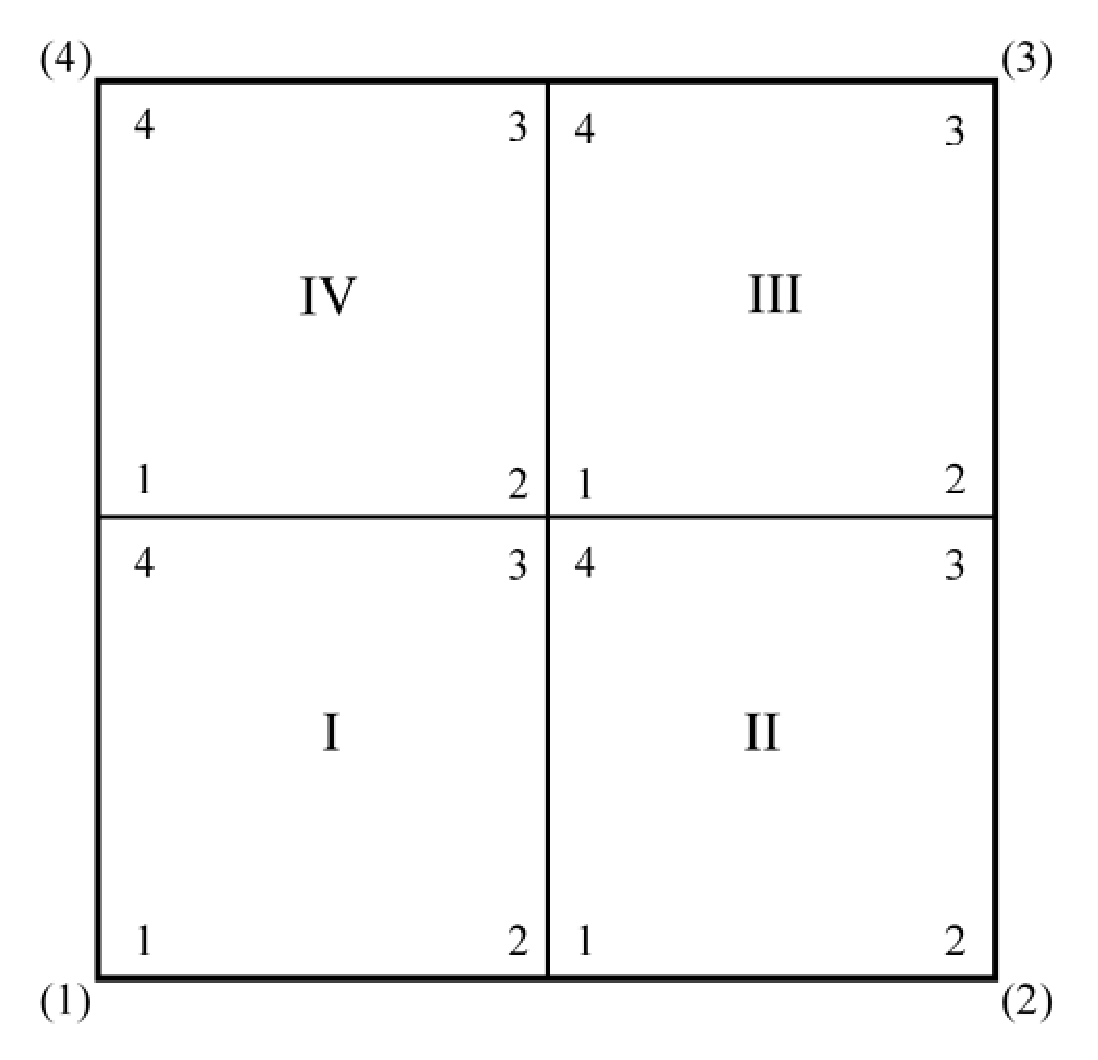
\includegraphics[width=0.45\textwidth]{figures/sec_Sn/Quad_cell_refinement_rules.eps}
\caption{Refinement rules for a quadrilateral mesh cell.}
\label{fig::Sn_Solution_Spatial_AMR_quadrefrules}
\end{figure}

Once a mesh element from level $r$ has been refined, we need to incorporate its daughter elements into the adapted mesh, $\mathbb{T}_h^{r+1}$. We can see from the nesting refinement process that these AMR procedures lead to a hierarchical representation of the mesh. All of the mesh cells are obtained by subdivisions of cells from the initial mesh, $\mathbb{T}_h^0$. This hierarchical nature of the mesh can succinctly be described in a tree structure. We give an example of this tree structure in Figure \ref{fig::Sn_Solution_Spatial_AMR_tree} for the simple case of a 2-cell domain that undergoes two refinement cycles with 1 cell refined per cycle. From the tree structure in Figure \ref{fig::Sn_Solution_Spatial_AMR_tree_struct}, we introduce the concept of an individual element's {\em refinement level}, $\ell(K)$, for mesh cell $K$. The refinement level $\ell(K)$ denotes how many times a cell from the original mesh, $\mathbb{T}_h^0$, has been refined to form element $K$. By convention, the refinement level for all elements in the original mesh is 0. We note that an element's refinement level is not necessarily the number of refinement cycles that have been performed. In Figure \ref{fig::Sn_Solution_Spatial_AMR_tree_struct}, we can see three distinct refinement levels that are represented by the three different vertical levels of nodes. Element 1 has a level of 0 since it was never refined. Elements 2, 3, 4, and 5 have a level of 2. Finally, elements 6, 7, and 8 have a level of 1. We also use Figure \ref{fig::Sn_Solution_Spatial_AMR_tree} to further define the concept of an {\em irregularity index}. This index is the difference in refinement levels between two adjoining mesh elements. The irregularity index for the face separating elements 6 and 7 is 0 since $\ell(6)=\ell(7)$. The irregularity index for the face separating elements 4 and 8 is 1 since $\ell(8)=1$ and $\ell(4)=2$. Finally, the irregularity index for the face separating elements 1 and 2 is 2 since $\ell(1)=0$ and $\ell(2)=2$. For the AMR problems in this work, we restrict the maximum allowable irregularity index for all of the elements for each of the mesh refinement levels.

\begin{figure}
\centering
{
	\begin{subfigure}[b]{0.48\textwidth}
		\centering
		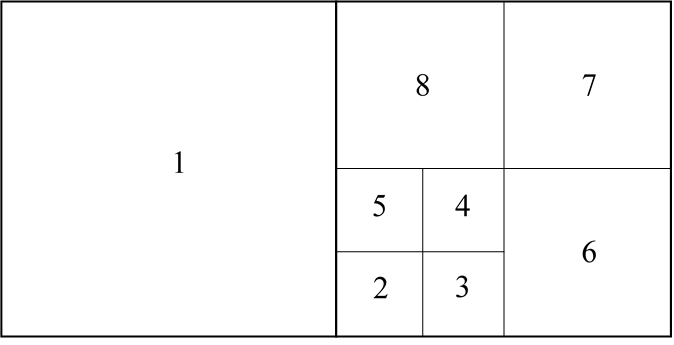
\includegraphics[width=0.95\textwidth]{figures/sec_Sn/Quad_tree_domain.png}
		\caption{Twice-refined domain}
		\label{fig::Sn_Solution_Spatial_AMR_tree_dom}
	\end{subfigure}
}
	\hfill
{
	\begin{subfigure}[b]{0.48\textwidth}
		\centering
		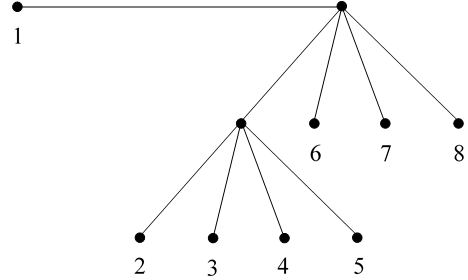
\includegraphics[width=0.85\textwidth]{figures/sec_Sn/Quad_tree_structure.png}
		\caption{Refinement tree structure}
		\label{fig::Sn_Solution_Spatial_AMR_tree_struct}
	\end{subfigure}
}
\caption{Hierarchical refinement tree for a simple domain with quadrilateral cells.}
\label{fig::Sn_Solution_Spatial_AMR_tree}
\end{figure}

Following a refinement cycle, we have a new adapted mesh, $\mathbb{T}_h^{r+1}$, but our current solution lives on $\mathbb{T}_h^{r}$. This means that the solution lives on a lower-dimensional space than the next solution on the newly adapted mesh. To solve for the transport solution on $\mathbb{T}_h^{r+1}$, we could simply reinitialize our solution vectors to zero and follow the procedures in Algorithm \ref{alg::Sn_Linear_Transport_Solve}. However, this means that the solution from mesh $\mathbb{T}_h^{r}$ would simply be discarded. This would discount all the work performed to compute the solution on level $r$. Furthermore, if there is little difference in the functional space between the two refinement cycles, then the calculated solution at level $r$ would be a good initial guess for the solution to be calculated for level $r+1$. For this reason, we define the concept of {\em bootstrapping}, which is the projection of the solution from $\mathbb{T}_h^{r}$ onto $\mathbb{T}_h^{r+1}$. Figure \ref{fig::Sn_Solution_Spatial_AMR_bootstrapping} provides an example of bootstrapping by refining a single unit square element onto the four identical daughter elements with $\frac{1}{4}$ the area as the parent element. Figure \ref{fig::Sn_Solution_Spatial_AMR_BS_before} shows a linear planar solution on a single unit square parent element. Then, after this element is refined, its solution is projected onto its four identical daughter elements. Figure \ref{fig::Sn_Solution_Spatial_AMR_BS_after} shows this bootstrapped solution onto the refined mesh, where we can clearly see that the projected solution lives in the dimensional space of the daughter elements but still lives in the functional space of the parent element.

\begin{figure}
\centering
{
	\begin{subfigure}[b]{0.48\textwidth}
		\centering
		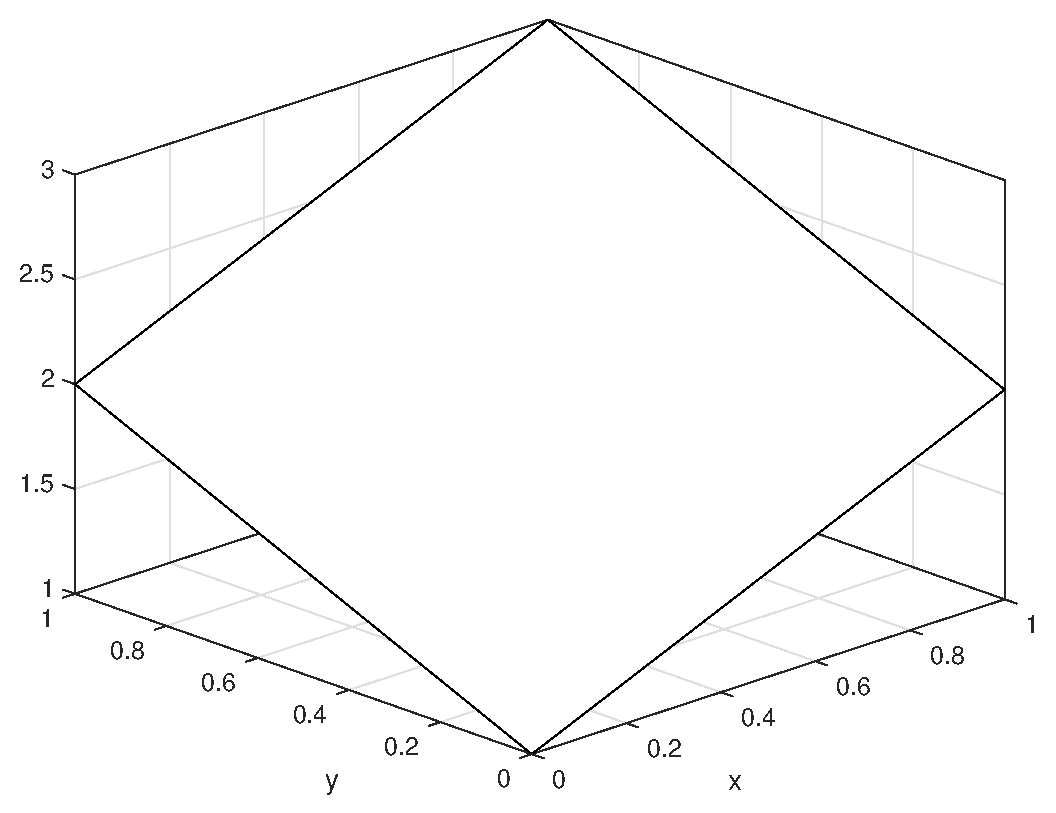
\includegraphics[width=0.95\textwidth]{figures/sec_Sn/cell_refinement_before.eps}
		\caption{Before refinement}
		\label{fig::Sn_Solution_Spatial_AMR_BS_before}
	\end{subfigure}
}
	\hfill
{
	\begin{subfigure}[b]{0.48\textwidth}
		\centering
		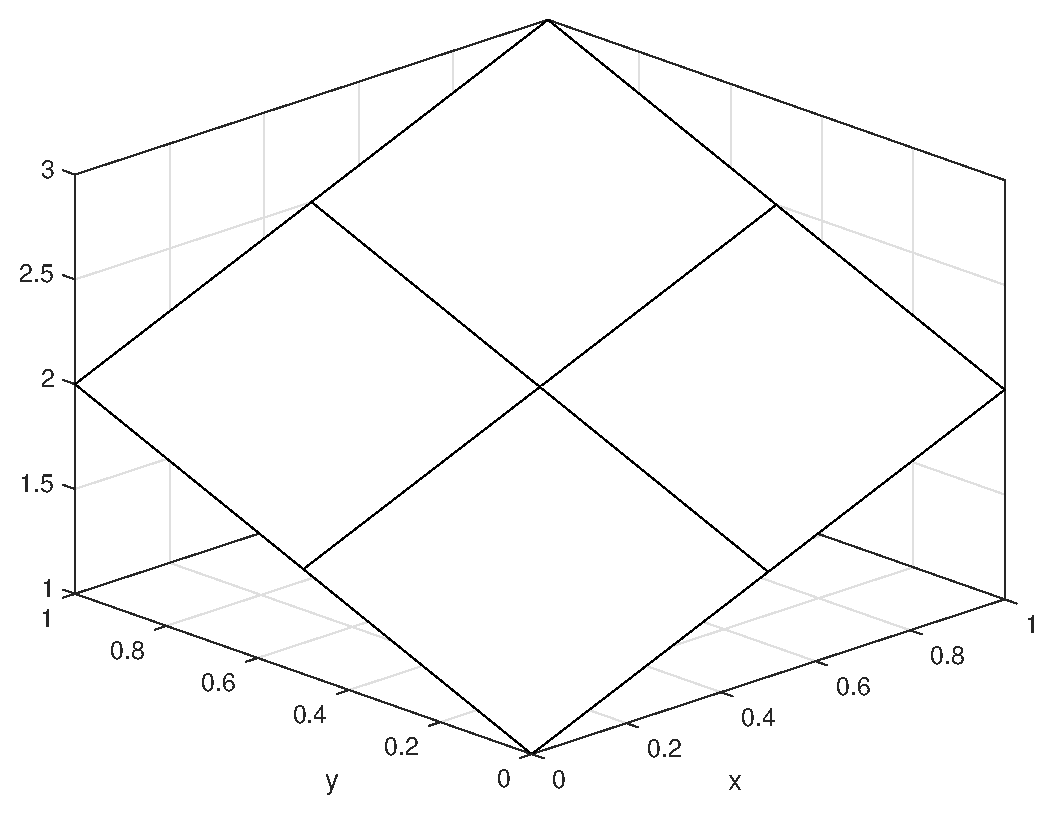
\includegraphics[width=0.95\textwidth]{figures/sec_Sn/cell_refinement_after.eps}
		\caption{After refinement}
		\label{fig::Sn_Solution_Spatial_AMR_BS_after}
	\end{subfigure}
}
\caption{Bootstrapping the solution from a single unit square element onto the four daughter elements after refinement.}
\label{fig::Sn_Solution_Spatial_AMR_bootstrapping}
\end{figure}

%%%%%%%%%%%%%%%%%%%%%%%%%%%%%%%%%%%%%%%%%%%%%%%%%%%
%%%   Section - Conclusions
\section{Conclusions}
\label{sec::Sn_Conclusions}

In this chapter, we have presented the tightly-coupled system of equations that comprise the DGFEM $S_N$ transport equation. We began with the fully-continuous transport equation presented in Section \ref{sec::Sn_neut} and then discretized it in energy, angle and space in Sections \ref{sec::Sn_MG}, \ref{sec::Sn_Angle}, and \ref{sec::Sn_Spatial}, respectively. Appropriate boundary conditions were presented in Section \ref{sec::Sn_BC}. For this work, we will only utilize incoming-incident and reflecting boundary conditions and not use any further albedo terms. We finished this chapter in Section \ref{sec::Sn_Solution} by describing the procedures that will be utilized to solve our system of equations in energy, angle, and space. We also provided the methodology that we will employ to perform AMR calculations in this work, which yields another mechanism to produce polytope meshes.

